\documentclass[conference]{IEEEtran}
\IEEEoverridecommandlockouts
\usepackage[utf8]{inputenc}
\usepackage[T1]{fontenc}
\usepackage[spanish,es-tabla,es-noshorthands,es-nodecimaldot]{babel}
\spanishplainpercent
\usepackage{amsmath,amssymb}
\usepackage{icomma}
\usepackage[output-decimal-marker={,},group-minimum-digits=5,per-mode=symbol]{siunitx}
\DeclareSIUnit{\VAr}{VAr}
\DeclareSIUnit{\rpm}{r/min}
\usepackage{pgfplots}
\pgfplotsset{compat=1.17}
\usepackage[caption=false,font=footnotesize]{subfig}
\usepackage{graphicx}
\usepackage{placeins}
\usepackage{booktabs}
\usepackage{xcolor}
\usepackage{xurl}
\usepackage{hyperref}
\hypersetup{colorlinks=true,linkcolor=black,citecolor=black,urlcolor=blue!50!black}

% ---------------------------------------------------------------------------
% Interruptor de borrador: en true muestra las notas internas (en rojo).
\newif\ifborrador
\borradorfalse
\newcommand{\nota}[1]{\ifborrador{\color{red}\footnotesize[#1]}\fi}
% ---------------------------------------------------------------------------

% Valores generados por los scripts de calculos/
\newcommand{\LVns}{\num{1800}}
\newcommand{\LVs}{\num{6.39}}
\newcommand{\LVfr}{\num{3.83}}
\newcommand{\LVS}{\num{410.7}}
\newcommand{\LVPin}{\num{299.8}}
\newcommand{\LVQin}{\num{280.7}}
\newcommand{\LVeta}{\num{66.7}}
\newcommand{\LVw}{\num{176.5}}
\newcommand{\LVT}{\num{1.133}}
\newcommand{\LVVfY}{\num{120.1}}
\newcommand{\LVIfD}{\num{1.97}}
\newcommand{\LVVlD}{\num{120.1}}
\newcommand{\LVperdidas}{\num{99.8}}
\newcommand{\TvGuiaA}{\num{240}}
\newcommand{\TvLVA}{\num{131.0}}
\newcommand{\TvPctA}{\num{109.1}}
\newcommand{\TvGuiaB}{\num{220}}
\newcommand{\TvLVB}{\num{120.1}}
\newcommand{\TvPctB}{\num{100.0}}
\newcommand{\TvGuiaC}{\num{200}}
\newcommand{\TvLVC}{\num{109.2}}
\newcommand{\TvPctC}{\num{90.9}}
\newcommand{\TvGuiaD}{\num{180}}
\newcommand{\TvLVD}{\num{98.3}}
\newcommand{\TvPctD}{\num{81.8}}
\newcommand{\TvGuiaE}{\num{160}}
\newcommand{\TvLVE}{\num{87.3}}
\newcommand{\TvPctE}{\num{72.7}}
\newcommand{\TvGuiaF}{\num{140}}
\newcommand{\TvLVF}{\num{76.4}}
\newcommand{\TvPctF}{\num{63.6}}
\newcommand{\TvGuiaG}{\num{120}}
\newcommand{\TvLVG}{\num{65.5}}
\newcommand{\TvPctG}{\num{54.5}}
\newcommand{\TvGuiaH}{\num{100}}
\newcommand{\TvLVH}{\num{54.6}}
\newcommand{\TvPctH}{\num{45.5}}
\newcommand{\LVsEstEighty}{\num{9.98}}
\newcommand{\LVnEstEighty}{\num{1620}}
\newcommand{\LVsEstSixty}{\num{17.75}}
\newcommand{\LVnEstSixty}{\num{1481}}
\newcommand{\LVR}{\num{14.0}}
\newcommand{\LVRY}{\num{28.0}}
\newcommand{\LVRD}{\num{9.33}}
\newcommand{\DLnsCinc}{\num{3000}}
\newcommand{\DLs}{\num{4.33}}
\newcommand{\DLfr}{\num{2.17}}
\newcommand{\DLnsSes}{\num{3600}}
\newcommand{\DLnSes}{\num{3444}}
\newcommand{\DLT}{\num{3.66}}
\newcommand{\DLSD}{\num{1639}}
\newcommand{\DLSY}{\num{1645}}
\newcommand{\DLIfD}{\num{2.48}}
\newcommand{\DLVfY}{\num{219.4}}
\newcommand{\DLtolA}{\num{3}}
\newcommand{\DLtolB}{\num{5}}
\newcommand{\DLfpeta}{\num{0.671}}
\newcommand{\DLdVD}{\num{230}}
\newcommand{\DLdVY}{\num{400}}
\newcommand{\DLdS}{\num{1732}}

\newcommand{\Rvi}{\num{14.19}}
\newcommand{\Rvimin}{\num{14.00}}
\newcommand{\Rvimax}{\num{14.18}}
\newcommand{\Rinter}{\num{-0.076}}
\newcommand{\Rdesv}{\num{0.00}}
\newcommand{\DdosVL}{\num{208.1}}
\newcommand{\DdosIL}{\num{3.46}}
\newcommand{\DdosIF}{\num{2.00}}
\newcommand{\DdosP}{\num{320}}
\newcommand{\Pmec}{\num{63.5}}
\newcommand{\kfe}{\num{0.909}}
\newcommand{\VnomVac}{\num{120.5}}
\newcommand{\InomVac}{\num{1.308}}
\newcommand{\PceroNom}{\num{100.4}}
\newcommand{\PcuNom}{\num{23.9}}
\newcommand{\ProtNom}{\num{76.4}}
\newcommand{\PfeNom}{\num{12.9}}
\newcommand{\FPnomVac}{\num{0.368}}
\newcommand{\Zvac}{\num{159.6}}
\newcommand{\Rfe}{\num{3366}}
\newcommand{\CnomI}{\num{1.980}}
\newcommand{\CnomT}{\num{1.056}}
\newcommand{\Cnomn}{\num{1673}}
\newcommand{\CnomPin}{\num{328.4}}
\newcommand{\CnomPout}{\num{185.0}}
\newcommand{\Cnometa}{\num{56.3}}
\newcommand{\Cnoms}{\num{7.06}}
\newcommand{\Cnomfp}{\num{0.797}}
\newcommand{\Cetamax}{\num{57.3}}
\newcommand{\Cultn}{\num{1649}}
\newcommand{\CultPout}{\num{215.5}}
\newcommand{\CultI}{\num{2.185}}
\newcommand{\Cults}{\num{8.39}}
\newcommand{\Culteta}{\num{57.3}}
\newcommand{\Cnvac}{\num{1773}}
\newcommand{\CRV}{\num{5.98}}
\newcommand{\CerrPm}{\num{0.07}}
\newcommand{\CnomPcuu}{\num{54.9}}
\newcommand{\CnomPag}{\num{260.5}}
\newcommand{\CnomPcud}{\num{18.4}}
\newcommand{\CnomResto}{\num{-6.4}}


% Parametros de flotantes para aprovechar mejor las paginas
\renewcommand{\topfraction}{0.9}
\renewcommand{\dbltopfraction}{0.9}
\renewcommand{\textfraction}{0.08}
\renewcommand{\floatpagefraction}{0.75}
\renewcommand{\dblfloatpagefraction}{0.75}
\setcounter{topnumber}{3}
\setcounter{dbltopnumber}{3}

\pgfplotsset{
  lab/.style={width=\columnwidth,height=0.62\columnwidth,grid=major,
    grid style={gray!25},tick label style={font=\footnotesize},
    label style={font=\footnotesize},legend style={font=\scriptsize},
    /pgf/number format/use comma,/pgf/number format/1000 sep={}},
}

\begin{document}

\title{Preinforme de Laboratorio: Práctica N.º 4 --- Máquinas de inducción}

\author{
\IEEEauthorblockN{Simón David Pinzón Navarro, Luisa Fernanda Marín Romero, Juan Andrés Merchán Palencia,\\
Johan Emanuel Pino Giraldo y Cristian Manuel Marquez Luna}
\IEEEauthorblockA{Programa de Ingeniería Eléctrica, Universidad del Norte, Barranquilla, Colombia}
}

\maketitle

\begin{abstract}
Este preinforme prepara la Práctica N.º 4 de Máquinas Eléctricas I, dedicada a los motores de inducción trifásicos. Se presentan las máquinas del banco físico (motor de jaula de ardilla De Lorenzo DL~1021 y motor de rotor devanado), el análisis de sus datos de placa, una aplicación industrial, los cálculos previos que pide la guía y la descripción de las conexiones de todas las actividades. Cada actividad se reprodujo en el simulador LVSIM-EMS con el motor de jaula LabVolt 8221, un dinamómetro 8960 y la interfaz de adquisición 9063. En el simulador la resistencia por fase resultó de \SI{14,0}{\ohm} (con \Rvi~\si{\ohm} por el método voltímetro-amperímetro); en vacío a \SI{120}{V} en delta el motor absorbe \PceroNom~\si{W}, de los cuales \PcuNom~\si{W} son pérdidas en el cobre del estator, \Pmec~\si{W} pérdidas mecánicas y \PfeNom~\si{W} pérdidas en el hierro; y con corriente nominal entrega \CnomPout~\si{W} a \Cnomn~\si{\rpm}, con deslizamiento de \Cnoms~\% y eficiencia de \Cnometa~\%. Los resultados confirman que el sentido de giro depende de la secuencia de fases, que la conexión delta a \SI{120}{V} equivale a la estrella a \SI{208}{V} y que el deslizamiento crece con la carga y al reducir la tensión.
\end{abstract}

\begin{IEEEkeywords}
motor de inducción, jaula de ardilla, rotor devanado, deslizamiento, prueba de vacío, prueba de carga, método de dos vatímetros, LVSIM-EMS.
\end{IEEEkeywords}

% ===========================================================================
\section{Introducción}
El motor de inducción trifásico es la máquina eléctrica más usada en la industria por su construcción robusta, su bajo costo y su mantenimiento mínimo \cite{chapman,fitzgerald}. Su principio es el de un transformador rotativo: el estator, alimentado con un sistema trifásico, crea un campo magnético giratorio que induce tensiones y corrientes en el rotor; la interacción entre esas corrientes y el campo produce el par que hace girar el eje \cite{guia,diapositivas}.

La Práctica N.º 4 \cite{guia} tiene dos actividades: la exploración de los motores (medida de resistencia de los devanados y puesta en operación de un motor de rotor devanado y uno de jaula de ardilla, en estrella y en delta) y las pruebas de vacío y de carga de un motor de jaula conectado en delta. Este documento prepara esa práctica: reseña de las máquinas, análisis de placa, cálculos previos, conexiones, montajes y simulación de cada actividad en LVSIM-EMS \cite{lvsim}. Los datos del laboratorio físico se analizarán en el informe final.

% ===========================================================================
\section{Objetivos}
Según la guía \cite{guia}, la práctica busca:
\begin{itemize}
\item Tener un acercamiento general a los motores de inducción y verificar sus aspectos constructivos y características básicas.
\item Medir la resistencia del estator como base para calcular las pérdidas en el cobre y las pérdidas rotacionales.
\item Determinar las pérdidas mecánicas (fricción y ventilación) y en el hierro (histéresis y corrientes parásitas), y comprobar que su suma con las del cobre es la potencia absorbida en vacío.
\item Determinar las características de operación, la regulación de velocidad y la eficiencia de un motor de inducción trifásico.
\item Estimar los parámetros del circuito equivalente del motor.
\end{itemize}
En este preinforme se agregan dos objetivos de preparación: anticipar con cálculos y simulación los valores esperados en el banco y fijar los límites que no se deben superar.

% ===========================================================================
\section{Reseña y fundamentos teóricos}

\subsection{Campo giratorio y velocidad sincrónica}
Tres devanados desplazados \SI{120}{\degree} eléctricos y alimentados con corrientes trifásicas balanceadas producen un campo de amplitud constante que gira a la velocidad sincrónica \cite{chapman}:
\begin{equation}
n_s=\frac{120\,f_e}{P},
\label{eq:ns}
\end{equation}
donde $f_e$ es la frecuencia de la red y $P$ el número de polos. A \SI{60}{Hz}, una máquina de 2 polos tiene $n_s=\SI{3600}{\rpm}$ y una de 4 polos, \SI{1800}{\rpm} \cite{diapositivas}. El sentido del campo lo fija la secuencia de fases: al intercambiar dos líneas se invierte la secuencia y, con ella, el sentido de giro.

\subsection{Par inducido y deslizamiento}
El campo del estator $\mathbf{B}_S$ corta los conductores del rotor e induce en ellos $e=(\mathbf{v}\times\mathbf{B})\cdot\mathbf{l}$. Si el circuito del rotor está cerrado circula una corriente que crea el campo $\mathbf{B}_R$, y el par es $\tau_{ind}=k\,\mathbf{B}_R\times\mathbf{B}_S$ \cite{diapositivas}. Para que haya tensión inducida debe existir movimiento relativo entre el campo y el rotor; por eso el rotor nunca alcanza $n_s$. Esa diferencia se mide con el deslizamiento:
\begin{equation}
s=\frac{n_s-n_m}{n_s},
\label{eq:s}
\end{equation}
y la frecuencia de las corrientes del rotor es
\begin{equation}
f_r=s\,f_e .
\label{eq:fr}
\end{equation}
Con el rotor bloqueado ($s=1$) la frecuencia y la tensión del rotor son máximas; a velocidad sincrónica ($s=0$) ambas serían nulas y no habría par \cite{diapositivas}. Si una máquina externa impulsa el rotor por encima de $n_s$, el deslizamiento se vuelve negativo, el par se invierte y la máquina trabaja como generador, aunque sigue consumiendo potencia reactiva para magnetizarse \cite{generador}.

\subsection{Rotor de jaula y rotor devanado}
El rotor de jaula de ardilla está formado por barras cortocircuitadas en sus extremos por anillos; no tiene bornes accesibles. El rotor devanado tiene un devanado trifásico, normalmente en estrella, cuyos terminales salen por anillos rozantes y escobillas \cite{chapman,guia}. Con los terminales del rotor abiertos no circula corriente rotórica y no hay par: el motor se comporta como un transformador en vacío y en los anillos aparece la tensión inducida a rotor bloqueado $E_{R0}$. Al cortocircuitarlos, el motor arranca como uno de jaula. El acceso al rotor permite insertar resistencias para mejorar el par de arranque y limitar la corriente, a costa de mayores pérdidas \cite{chapman,generador}.

\subsection{Circuito equivalente y flujo de potencia}
Por fase, el motor se representa con la resistencia y reactancia del estator ($R_1$, $X_1$), la rama de magnetización ($R_c\parallel jX_M$) y el rotor referido al estator ($R_2/s$, $X_2$) \cite{chapman,fitzgerald}. La potencia de entrada se reparte así:
\begin{gather}
P_{in}=P_{Cu1}+P_{n\acute{u}cleo}+P_{AG},\qquad P_{Cu2}=s\,P_{AG},\label{eq:flujo1}\\
P_{conv}=(1-s)P_{AG},\qquad P_{out}=P_{conv}-P_{mec}-P_{misc}.\label{eq:flujo2}
\end{gather}
En vacío $P_{out}=0$ y el deslizamiento es tan pequeño que $P_{Cu2}\approx 0$; por eso la potencia absorbida cubre solo el cobre del estator, el núcleo y las pérdidas mecánicas. Esa es la base de la prueba de vacío \cite{guia,ieee112}.

\subsection{Curva par-velocidad y clases de diseño}
El par crece casi linealmente con el deslizamiento cerca de $n_s$, llega a un máximo (par de desenganche) y luego cae. A deslizamiento fijo el par es proporcional a $V^2$, por lo que una reducción de tensión aumenta el deslizamiento para un mismo par de carga \cite{chapman}. Las clases NEMA A, B, C y D difieren en par de arranque, corriente de arranque y deslizamiento nominal; las clases A y B tienen deslizamientos a plena carga menores al \SI{5}{\percent} \cite{diapositivas}.

% ===========================================================================
\section{Máquinas y equipos}

\subsection{Banco físico}
La guía usa dos motores \cite{guia}:
\begin{itemize}
\item \textbf{Motor de inducción trifásico de jaula de ardilla De Lorenzo DL~1021} (Fig.~\ref{fig:equipos}a), con estator trifásico de seis bornes y jaula embebida en el rotor \cite{dl1021}.
\item \textbf{Motor de inducción trifásico de rotor devanado.} La guía no da su referencia. Se supone el De Lorenzo DL~1022 (Fig.~\ref{fig:equipos}b), el motor de anillos de la misma línea, con devanados trifásicos en estator y rotor \cite{dl1022}.
\end{itemize}
Completan el banco la fuente trifásica variable, voltímetros, amperímetros o pinza amperimétrica, vatímetro trifásico, tacómetro, fuente de corriente continua y freno electromagnético con brazo y pesa para la prueba de carga \cite{guia}. La Fig.~\ref{fig:equipos}c muestra el interior de un motor de jaula: el estator bobinado y el rotor con su paquete de chapas.

\begin{figure}[!t]
\centering
\subfloat[]{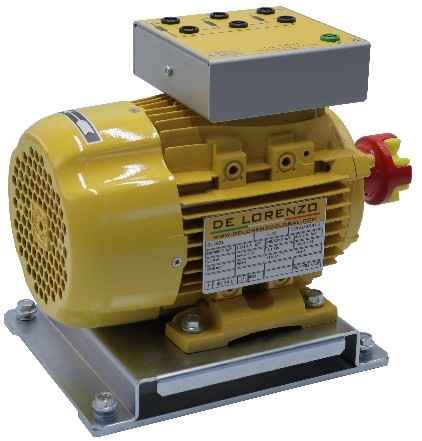
\includegraphics[height=0.33\columnwidth]{figuras/equipos/dl1021.jpg}}\hfill
\subfloat[]{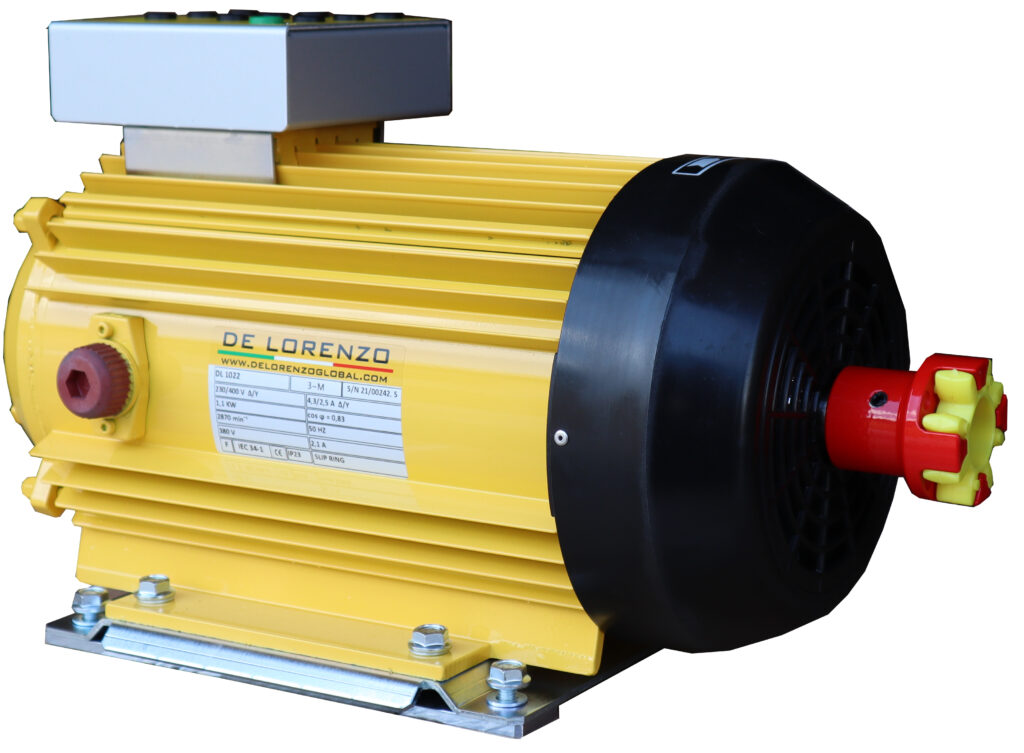
\includegraphics[height=0.33\columnwidth]{figuras/equipos/dl1022.jpg}}\\[2pt]
\subfloat[]{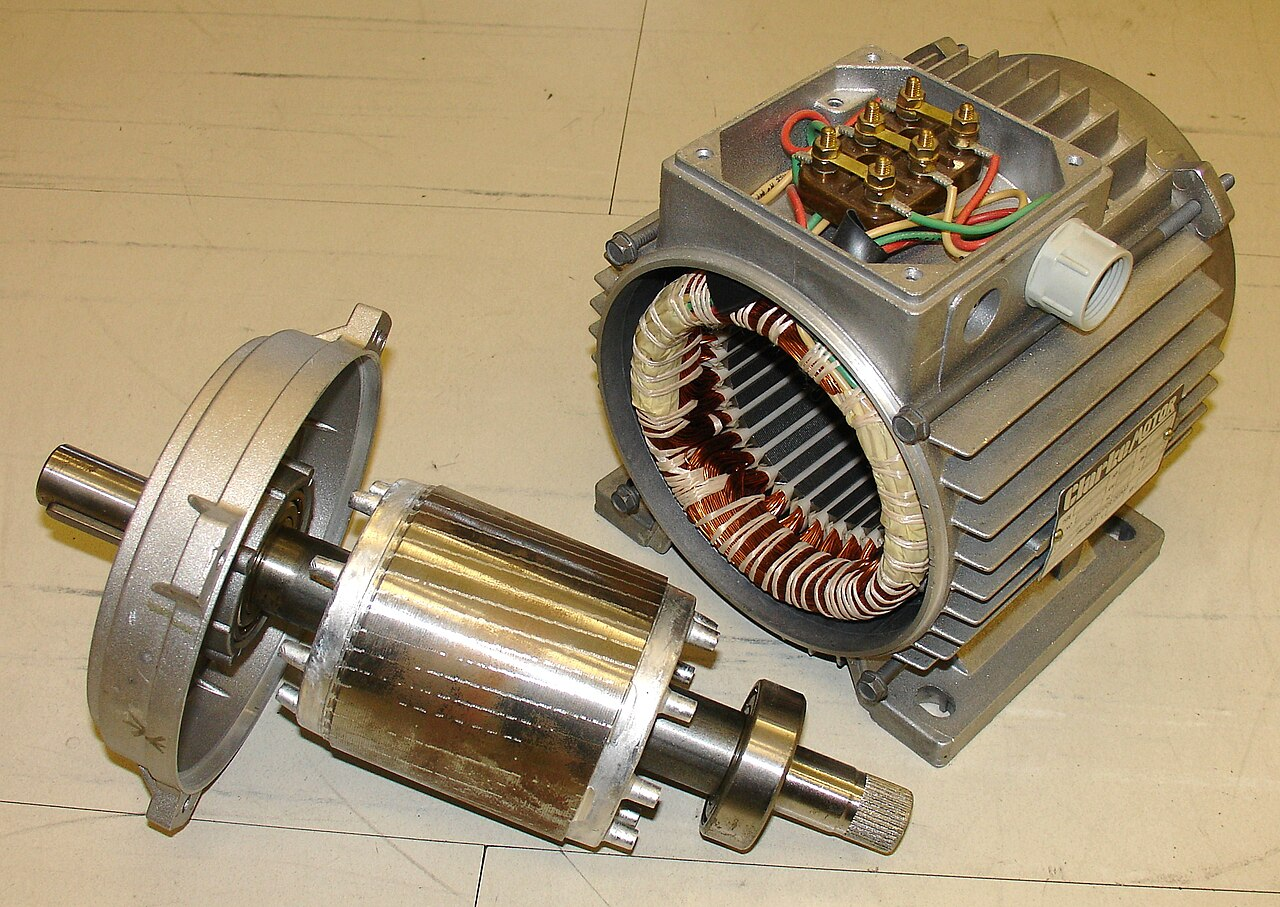
\includegraphics[width=0.72\columnwidth]{figuras/equipos/estator_rotor.jpg}}
\caption{Máquinas del banco físico. (a) Motor de jaula De Lorenzo DL~1021 \cite{dl1021}. (b) Motor de rotor devanado De Lorenzo DL~1022 \cite{dl1022}. (c) Estator y rotor de jaula de un motor de inducción desarmado \cite{img_estator}.}
\label{fig:equipos}
\end{figure}

\subsection{Equipos del simulador LVSIM-EMS}
LVSIM-EMS \cite{lvsim} reproduce el sistema electromecánico LabVolt. Para esta práctica se usaron (Fig.~\ref{fig:lvsimmod}):
\begin{itemize}
\item Motor de inducción de jaula de ardilla de cuatro polos 8221-02: \SI{208}{V}, 3$\phi$, \SI{60}{Hz}; como motor, \SI{200}{W}, FP~0,73, \SI{1685}{\rpm}, \SI{1,14}{A}; cada bobina del estator está marcada \SI{120}{V}--\SI{1,5}{A} \cite{lv8221}.
\item Motor de impulsión/dinamómetro 8960: en modo dinamómetro actúa como freno de par regulable (0--\SI{3}{N.m}, 0--\SI{2500}{\rpm}, \SI{175}{W} como dinamómetro) y entrega salidas analógicas de par y velocidad. Hace el papel del freno electromagnético y del tacómetro.
\item Fuente de alimentación 8821-02: salidas fija \num{120}/\SI{208}{V} y variable 0--\num{120}/\SI{208}{V}, \SI{5}{A}; salida de CC variable 0--\SI{120}{V}; salida de \SI{24}{V} CA.
\item Interfaz de adquisición de datos y control 9063 (DAI): cuatro entradas de tensión (E1--E4), cuatro de corriente (I1--I4) y entradas analógicas de par y velocidad. Con la ventana \emph{Aparatos de medición} cumple las funciones de voltímetros, amperímetros, vatímetros y tacómetro.
\item Multímetros virtuales amarillo y rojo, en función de óhmetro.
\end{itemize}

LVSIM no incluye un motor de rotor devanado. Por eso los pasos de la guía que dependen de los bornes del rotor se tratan desde la teoría (Sección~\ref{sec:analisis}) y en el banco físico se harán con el motor de anillos.

\begin{figure}[!t]
\centering
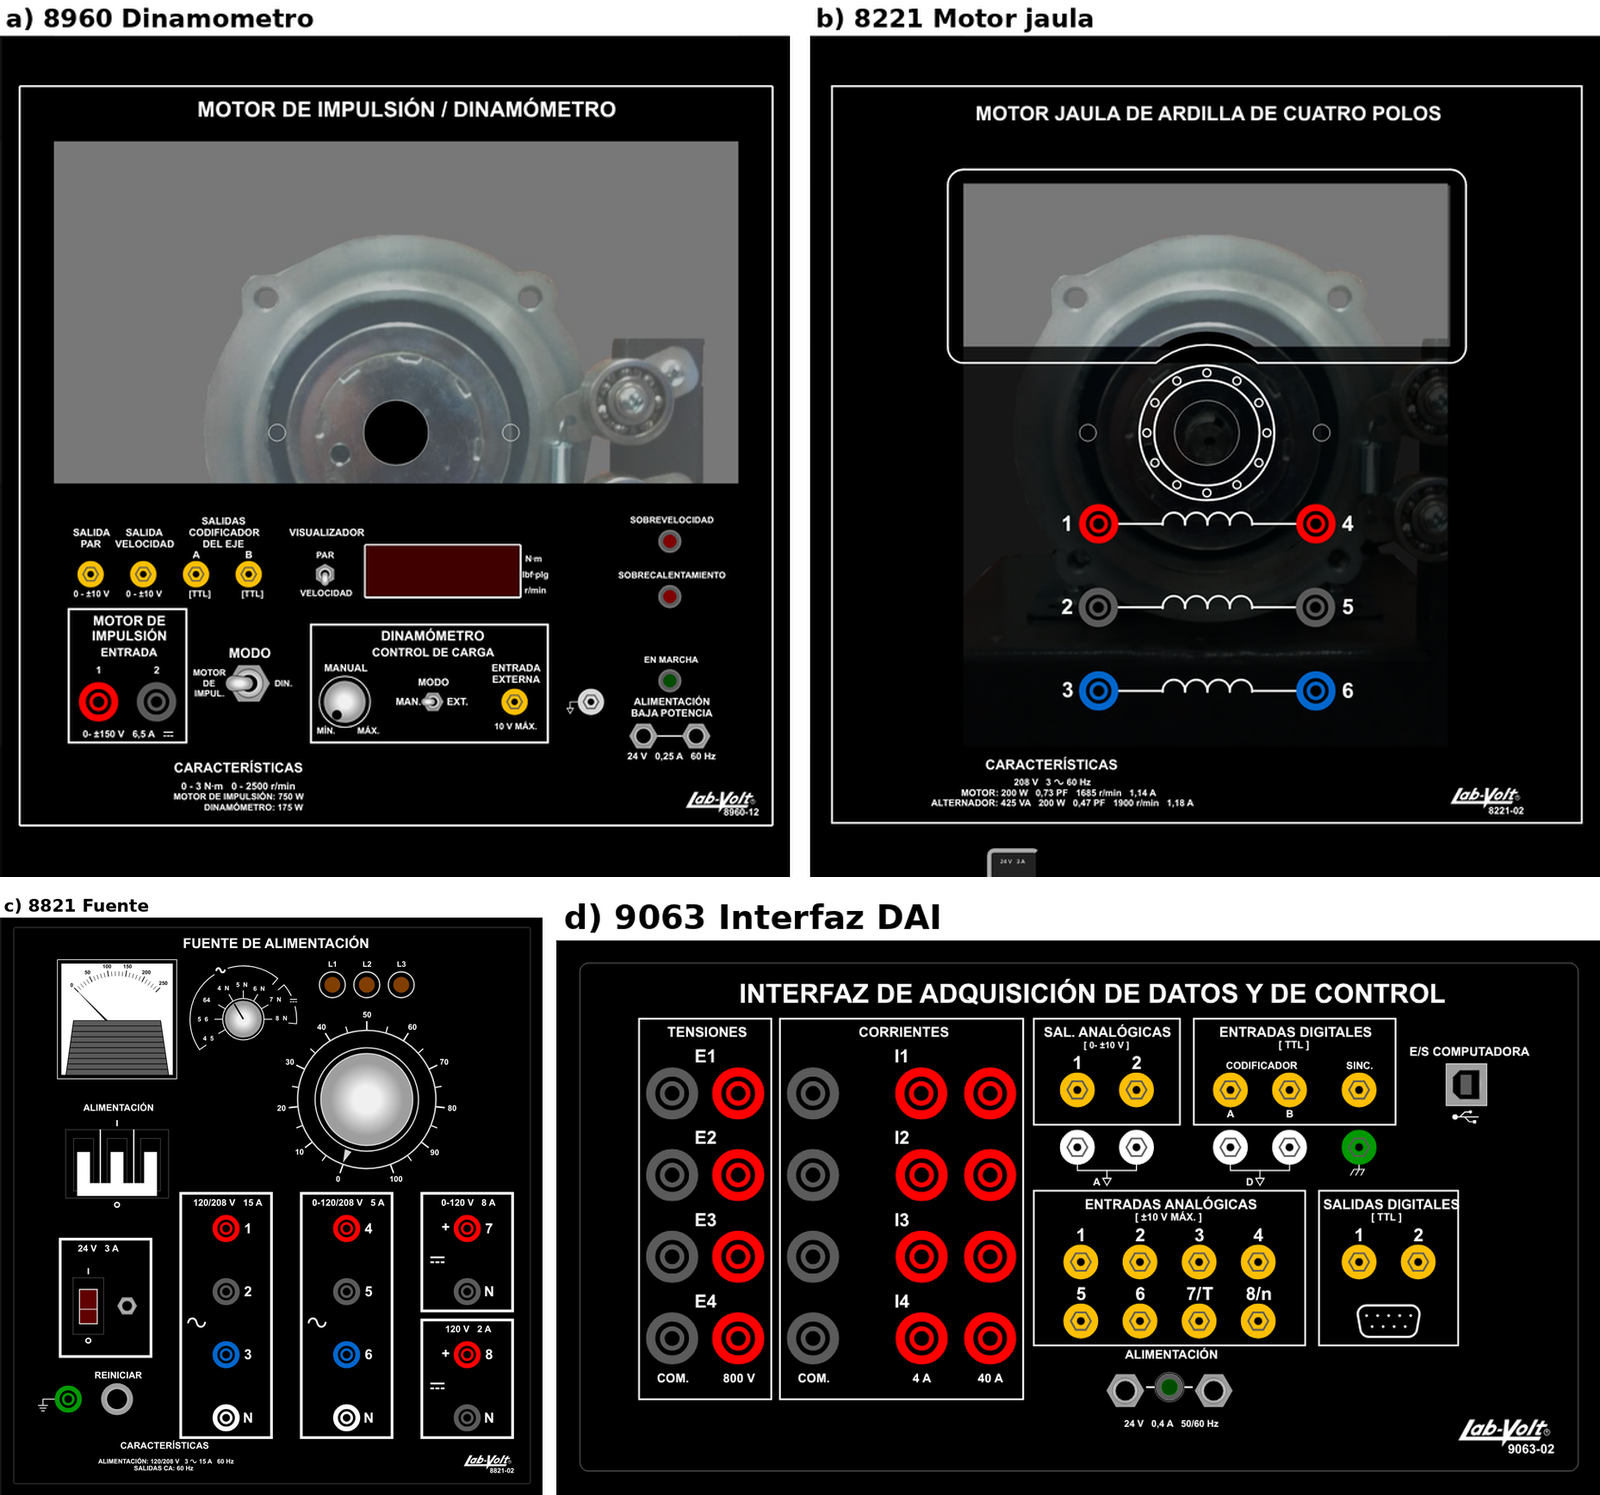
\includegraphics[width=\columnwidth]{figuras/lvsim/equipos_lvsim.png}
\caption{Módulos de LVSIM-EMS usados en las simulaciones, capturados del simulador \cite{lvsim}: (a) motor de impulsión/dinamómetro 8960, (b) motor de jaula 8221, (c) fuente 8821, (d) interfaz de adquisición 9063.}
\label{fig:lvsimmod}
\end{figure}

\IfFileExists{tablas/tabla_usuario.tex}{\input{tablas/tabla_usuario.tex}}{\nota{Aquí va la tabla que entrega Simón (tablas/tabla\_usuario.tex).}}

% ===========================================================================
\section{Análisis de la placa de características}

\subsection{Motor de jaula DL~1021}
El catálogo del fabricante \cite{dl1021} da los datos de la Tabla~\ref{tab:placadl}. Son datos de catálogo; deben confirmarse con la placa del motor del banco antes de la práctica.

\begin{table}[!t]
\centering
\caption{Datos de catálogo del DL~1021 e inferencias}
\label{tab:placadl}
\footnotesize
\begin{tabular}{@{}p{0.27\columnwidth}p{0.22\columnwidth}p{0.42\columnwidth}@{}}
\toprule
Dato & Valor & Inferencia \\
\midrule
Potencia & \SI{1,1}{kW} & Potencia mecánica en el eje; par nominal $\approx$ \DLT~\si{N.m} a \SI{2870}{\rpm}. \\
Tensión & \num{220}/\SI{380}{V} $\Delta$/Y & Bobina de \SI{220}{V}: delta en red de \SI{220}{V}, estrella en red de \SI{380}{V}. Las Tablas 20 y 21 de la guía usan delta. \\
Corriente & \num{4,3}/\SI{2,5}{A} $\Delta$/Y & En delta la corriente de fase es $4{,}3/\sqrt3=\DLIfD$~\si{A}, igual a la de estrella: la bobina trabaja igual en ambas conexiones. \\
Velocidad & \SI{2870}{\rpm}, \SI{50}{Hz} & $n_s=\DLnsCinc$~\si{\rpm}: 2 polos. $s=\DLs$~\%, $f_r=\DLfr$~\si{Hz}. A \SI{60}{Hz}, $n_s=\DLnsSes$~\si{\rpm} y $n\approx\DLnSes$~\si{\rpm}. \\
Potencia aparente & --- & $S=\sqrt3\,V_LI_L=\DLSD$~\si{VA} en delta (igual en estrella). \\
FP y eficiencia & no indicados & $\eta\cdot FP=P/S=\DLfpeta$; no se pueden separar sin la placa real. \\
\bottomrule
\end{tabular}
\end{table}

Tres inferencias son importantes para la práctica. Primera: como el banco opera a \SI{60}{Hz} y el catálogo está a \SI{50}{Hz}, la velocidad en vacío del DL~1021 será cercana a \SI{3600}{\rpm}, no a \SI{3000}{\rpm}; la nota del fabricante advierte una diferencia de alrededor del \SI{20}{\percent} \cite{dl1021}. Segunda: el motor admite las dos conexiones de la guía (estrella y delta) con tensiones de línea distintas; conectar en delta a la tensión de la estrella sometería cada bobina a $\sqrt3$ veces su tensión. Tercera: la corriente nominal en delta (\SI{4,3}{A}) es el límite de la prueba de carga.

\subsection{Motor de rotor devanado (DL~1022 supuesto)}
El catálogo del DL~1022 \cite{dl1022} indica \SI{1,1}{kW}, \num{230}/\SI{400}{V} $\Delta$/Y, \num{4,3}/\SI{2,5}{A} y \SI{2870}{\rpm} a \SI{50}{Hz}. Los mismos cálculos que para el DL~1021 dan 2 polos, $s=\DLs$~\% y $S\approx\DLdS$~\si{VA}. El catálogo no da la tensión del rotor ni la relación de transformación, por lo que la tensión en los anillos con rotor abierto se medirá en el banco.

\subsection{Motor LabVolt 8221 (LVSIM)}
La placa del módulo es: \SI{208}{V}, 3$\phi$, \SI{60}{Hz}; motor: \SI{200}{W}, FP~0,73, \SI{1685}{\rpm}, \SI{1,14}{A}; alternador: \SI{425}{VA}, \SI{200}{W}, FP~0,47, \SI{1900}{\rpm}, \SI{1,18}{A}. De ahí:
\begin{itemize}
\item $n_s=\LVns$~\si{\rpm} (4 polos); $s=\LVs$~\% y $f_r=\LVfr$~\si{Hz} a plena carga.
\item $S=\sqrt3(208)(1{,}14)=\LVS$~\si{VA}, $P_{in}=S\cdot FP=\LVPin$~\si{W}, $Q=\LVQin$~\si{\VAr} y $\eta=200/\LVPin=\LVeta$~\%.
\item $\tau_n=P/\omega=200/\LVw=\LVT$~\si{N.m}.
\item Cada bobina está marcada \SI{120}{V}. Los \SI{208}{V} de placa corresponden a la conexión en estrella ($208/\sqrt3=\LVVfY$~\si{V} por bobina). En delta la tensión nominal de línea es \SI{120}{V} y la corriente de línea nominal $1{,}14\sqrt3=\LVIfD$~\si{A}.
\item Los datos de alternador (\SI{1900}{\rpm} $>n_s$, FP~0,47) muestran que la misma máquina genera con deslizamiento negativo y que, aun generando, consume reactivos \cite{generador}.
\end{itemize}

% ===========================================================================
\section{Aplicación práctica}
Una aplicación típica del motor de jaula es el accionamiento de bombas centrífugas en acueductos, plantas de tratamiento, distritos de riego y sistemas de enfriamiento industrial. La Fig.~\ref{fig:aplicacion} muestra una bomba centrífuga normalizada acoplada a un motor de inducción con variador de frecuencia montado sobre la carcasa \cite{img_ksb}.

La elección del motor de inducción se justifica con las mismas características que se estudian en la práctica. Su velocidad casi constante (deslizamiento de pocos por ciento) mantiene el caudal estable aunque la carga hidráulica cambie. La jaula de ardilla no tiene escobillas ni anillos, lo que reduce el mantenimiento en ambientes húmedos. El variador cambia la frecuencia y, por la ecuación~\eqref{eq:ns}, la velocidad sincrónica; como la potencia de una bomba centrífuga varía aproximadamente con el cubo de la velocidad, una reducción moderada de velocidad produce un ahorro grande de energía frente al estrangulamiento con válvulas. Además, el variador limita la corriente de arranque, que en arranque directo es de 5 a 8 veces la nominal \cite{diapositivas}. La misma máquina, impulsada por encima de $n_s$, se usa como generador en aerogeneradores de velocidad fija tipo~A, como se vio en el material de apoyo \cite{generador}.

\begin{figure}[!t]
\centering
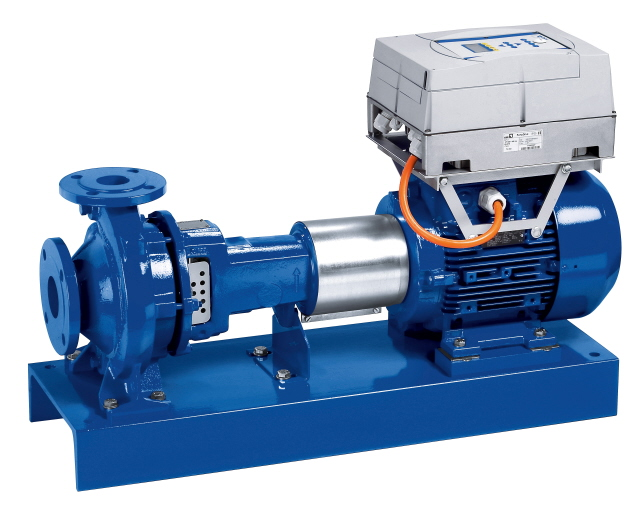
\includegraphics[width=0.85\columnwidth]{figuras/equipos/ksb_etanorm.jpg}
\caption{Bomba centrífuga accionada por un motor de inducción trifásico con variador de frecuencia integrado. Imagen: KSB AG, CC BY-SA 3.0 \cite{img_ksb}.}
\label{fig:aplicacion}
\end{figure}

% ===========================================================================
\section{Cálculos previos}
Los cálculos se reproducen con \texttt{calculos/calculos\_previos.py}, que escribe los valores en \texttt{calculos/salidas/previos.tex}.

\subsection{Velocidad sincrónica, deslizamiento y frecuencia del rotor}
Con \eqref{eq:ns}--\eqref{eq:fr}:
\begin{align*}
\text{DL 1021:}\;& n_s=\tfrac{120\cdot50}{2}=\DLnsCinc~\si{\rpm},\\
& s=\tfrac{3000-2870}{3000}=\DLs~\%,\quad f_r=\DLfr~\si{Hz};\\
\text{8221:}\;& n_s=\tfrac{120\cdot60}{4}=\LVns~\si{\rpm},\\
& s=\tfrac{1800-1685}{1800}=\LVs~\%,\quad f_r=\LVfr~\si{Hz}.
\end{align*}

\subsection{Par, potencia de entrada y eficiencia nominales}
Para el 8221: $\omega=1685\cdot2\pi/60=\LVw$~\si{rad/s}, $\tau_n=\LVT$~\si{N.m}, $S=\LVS$~\si{VA}, $P_{in}=\LVPin$~\si{W}, $\eta=\LVeta$~\%, y pérdidas totales a plena carga $P_{in}-P_{out}=\LVperdidas$~\si{W}. Para el DL~1021: $\tau_n=\DLT$~\si{N.m} y $S=\DLSD$~\si{VA}.

\subsection{Resistencia esperada entre líneas}
Si $R$ es la resistencia de una bobina, la medida entre dos líneas es $2R$ en estrella y $R\parallel 2R=2R/3$ en delta. Con $R=\LVR$~\si{\ohm} (valor del 8221 en LVSIM): \LVRY~\si{\ohm} en estrella y \LVRD~\si{\ohm} en delta. La guía fija una tolerancia del \DLtolA\,--\,\DLtolB~\% entre fases \cite{guia}.

\subsection{Tensiones de la prueba de vacío}
La Tabla~20 de la guía barre de \SI{240}{V} a \SI{100}{V} en delta, es decir, del \TvPctA~\% al \TvPctH~\% de los \SI{220}{V} nominales del DL~1021. En LVSIM, con \SI{120}{V} nominales en delta, se usaron las mismas fracciones (Tabla~\ref{tab:tensiones}).

\begin{table}[!t]
\centering
\caption{Tensiones de la prueba de vacío: guía y LVSIM}
\label{tab:tensiones}
\scriptsize
\setlength{\tabcolsep}{2.6pt}
\begin{tabular}{@{}lcccccccc@{}}
\toprule
Guía [V] & \TvGuiaA & \TvGuiaB & \TvGuiaC & \TvGuiaD & \TvGuiaE & \TvGuiaF & \TvGuiaG & \TvGuiaH\\
\% de $V_n$ & \TvPctA & \TvPctB & \TvPctC & \TvPctD & \TvPctE & \TvPctF & \TvPctG & \TvPctH\\
LVSIM [V] & \TvLVA & \TvLVB & \TvLVC & \TvLVD & \TvLVE & \TvLVF & \TvLVG & \TvLVH\\
\bottomrule
\end{tabular}
\end{table}

\subsection{Fórmulas de las pruebas de vacío y de carga}
Con el método de los dos vatímetros (conexión Aron) la potencia trifásica es $P_0=P_{W1}+P_{W2}$; uno de los vatímetros marca negativo cuando $FP<0{,}5$ \cite{fitzgerald}. En delta la corriente de fase es $I_\phi=I_L/\sqrt3$ y
\begin{gather}
P_{Cu}=3R_{est}I_\phi^2,\qquad P_m+P_{fe}=P_0-P_{Cu},\label{eq:pvacio}\\
\cos\theta=\frac{P_0}{\sqrt3\,V_LI_L}.\label{eq:fp}
\end{gather}
Las pérdidas en el hierro son casi proporcionales a $V^2$ y las mecánicas dependen solo de la velocidad, que en vacío es casi constante. Al graficar $P_m+P_{fe}$ contra $V^2$ y extrapolar a $V=0$ se obtienen las pérdidas mecánicas \cite{ieee112}. En la prueba de carga:
\begin{gather}
P_{out}=\tau\,\omega=\tau\frac{2\pi n}{60},\qquad \eta=\frac{P_{out}}{P_{in}}\times100,\label{eq:eta}\\
RV=\frac{n_{vac}-n_{pc}}{n_{pc}}\times100 .\label{eq:rv}
\end{gather}
En el freno físico el par se obtiene del equilibrio del brazo, $\tau=m\,g\,X$, con $X$ el desplazamiento de la pesa \cite{guia}. La masa de la pesa no aparece en la guía y se debe leer en el banco.

\subsection{Velocidad esperada con tensión reducida}
Con par de carga constante y $s$ pequeño, $\tau\propto V^2 s$, de modo que $s\propto1/V^2$. Partiendo del deslizamiento nominal del 8221, al \SI{80}{\percent} de la tensión se espera $s\approx\LVsEstEighty$\,\% y al \SI{60}{\percent}, $s\approx\LVsEstSixty$\,\%. En vacío el par de carga es solo el de fricción, de modo que los deslizamientos reales serán mucho menores; la tendencia (más deslizamiento con menos tensión) es la que se debe verificar.

% ===========================================================================
\section{Conexiones entre equipos}
\label{sec:conexiones}
En todo el documento, U1--U2, V1--V2 y W1--W2 son los extremos de las tres bobinas del estator. En el 8221 corresponden a los bornes 1--4, 2--5 y 3--6; los bornes 1, 2 y 3 tienen la misma polaridad instantánea.

\subsection{Actividad 1.1: resistencia de los devanados}
\begin{itemize}
\item \textbf{Óhmetro, por fase:} motor desenergizado y sin puentes. Terminal COM del óhmetro a U1 y terminal V$\Omega$ a U2; luego V1--V2 y W1--W2. En el motor de rotor devanado se repite en el estator y entre los anillos del rotor (K--L, L--M, K--M).
\item \textbf{Comprobación entre líneas:} con los puentes de estrella (U2--V2--W2) se mide entre U1 y V1; con los de delta se repite la medida.
\item \textbf{Voltímetro-amperímetro (opcional, en CC):} borne + de la fuente de CC variable a la entrada de un amperímetro; salida del amperímetro a U1; U2 al borne N de la fuente. Voltímetro en paralelo entre U1 (+) y U2 (--). La corriente se limita a menos de la nominal de la bobina.
\end{itemize}

\subsection{Actividad 1.2: puesta en operación}
\begin{itemize}
\item \textbf{Estrella:} puentes U2--V2--W2. Líneas L1, L2 y L3 de la fuente variable a U1, V1 y W1, cada una a través de un amperímetro (o abrazadas por la pinza). Voltímetro entre L1 y L2.
\item \textbf{Delta:} puentes U2--V1, V2--W1 y W2--U1. Las líneas entran por U1, V1 y W1 como en estrella.
\item \textbf{Rotor devanado:} los anillos K, L y M quedan primero abiertos con un voltímetro entre dos de ellos; luego se unen en un solo nodo con dos puentes (K--L y L--M).
\item \textbf{Inversión de giro:} con la fuente apagada se intercambian dos conductores de línea (L1$\leftrightarrow$L2) y, en el paso siguiente, otros dos (L2$\leftrightarrow$L3).
\item \textbf{Velocidad:} tacómetro óptico sobre el eje o, en LVSIM, salida de velocidad del dinamómetro acoplado por correa.
\end{itemize}

\subsection{Actividad 2: vacío y carga (delta)}
\begin{itemize}
\item \textbf{Fuente y corrientes:} L1, L2 y L3 de la fuente variable a U1, V1 y W1 a través de tres amperímetros. Estator en delta como en la actividad anterior.
\item \textbf{Vatímetro trifásico o dos vatímetros (Aron):} W1 con su bobina de corriente en la línea 1 y su bobina de tensión entre L1 (+) y L3; W2 con su bobina de corriente en la línea 2 y tensión entre L2 (+) y L3. Un voltímetro entre L1 y L2.
\item \textbf{Carga (prueba de carga):} eje del motor acoplado al freno electromagnético; el devanado del freno se alimenta de la fuente de CC a través de un amperímetro, y su corriente fija el par. En LVSIM, el dinamómetro 8960 acoplado por correa, en modo DIN. y control manual.
\end{itemize}

\subsection{Conexiones usadas en LVSIM}
Las conexiones de las simulaciones siguen lo anterior, con la DAI 9063 como instrumentación (Tabla~\ref{tab:conexlv}). Los cables se colorearon por fase: naranja (A), verde (B) y azul (C); los puentes de estrella y delta, en blanco en la actividad 1.1; las señales de par y velocidad, en amarillo.

\begin{table}[!t]
\centering
\caption{Conexiones de las simulaciones en LVSIM (actividades 1.2 y 2)}
\label{tab:conexlv}
\footnotesize
\begin{tabular}{@{}p{0.36\columnwidth}p{0.56\columnwidth}@{}}
\toprule
Desde & Hacia \\
\midrule
Fuente 4 (L1) & I1 (+) de la DAI; I1 (--) al borne 1 del motor \\
Fuente 5 (L2) & I2 (+); I2 (--) al borne 2 \\
Fuente 6 (L3) & I3 (+); I3 (--) al borne 3 \\
Puentes Y & 4--5 y 5--6 \\
Puentes $\Delta$ & 4--2, 5--3 y 6--1 \\
E1 (W1) & + al borne 1, -- al borne 3 ($V_{AC}$) \\
E2 (W2) & + al borne 2, -- al borne 3 ($V_{BC}$) \\
E3 & + al borne 1, -- al borne 2 ($V_{AB}$) \\
Dinamómetro par / velocidad & entradas analógicas 7/T y 8/n de la DAI; común a común \\
Fuente 24 V CA & alimentación de la DAI; el dinamómetro, con su adaptador de 24 V \\
Medidores & PQS1(E1,I1)=$P_{W1}$, PQS2(E2,I2)=$P_{W2}$, T, n, Pm(T,n) \\
\bottomrule
\end{tabular}
\end{table}

\subsection{Montajes físicos}
\IfFileExists{figuras/montajes/montajes.pdf}{La Fig.~\ref{fig:montajes} presenta}{Se preparan}\ los montajes sobre fotografías de los equipos del laboratorio, uno por actividad: (a) medida de resistencia, (b) puesta en operación del motor de rotor devanado, (c) puesta en operación del motor de jaula y (d) pruebas de vacío y de carga con freno.

\IfFileExists{figuras/montajes/montajes.pdf}{%
\begin{figure*}[p]
\centering
\subfloat[Actividad 1.1: resistencia de devanados.]{\includegraphics[width=0.48\textwidth,page=1]{figuras/montajes/montajes.pdf}}\hfill
\subfloat[Actividad 1.2: motor de rotor devanado.]{\includegraphics[width=0.48\textwidth,page=2]{figuras/montajes/montajes.pdf}}\\
\subfloat[Actividad 1.2: motor de jaula DL~1021.]{\includegraphics[width=0.48\textwidth,page=3]{figuras/montajes/montajes.pdf}}\hfill
\subfloat[Actividad 2: vacío y carga con freno.]{\includegraphics[width=0.48\textwidth,page=4]{figuras/montajes/montajes.pdf}}
\caption{Montajes físicos de la práctica sobre fotografías de los equipos.}
\label{fig:montajes}
\end{figure*}}{%
\ifborrador
\begin{figure*}[p]
\centering
\fbox{\parbox[c][0.8\textheight][c]{0.95\textwidth}{\centering\color{red} Montajes físicos (PDF de Simón): a) 1.1, b) 1.2 rotor devanado, c) 1.2 jaula, d) 2 vacío/carga}}
\caption{Montajes físicos de la práctica sobre fotografías de los equipos.}
\label{fig:montajes}
\end{figure*}
\fi}

% ===========================================================================
\section{Simulación en LabVolt (LVSIM-EMS)}
\label{sec:sim}

\subsection{Condiciones y adaptaciones}
Las simulaciones se hicieron en LVSIM-EMS \cite{lvsim} con red de \SI{120}{V}/\SI{60}{Hz}, los módulos de la Fig.~\ref{fig:lvsimmod} y una distribución propia del banco en cada actividad. Las lecturas son corridas reales del simulador: cada punto es el promedio de cinco o seis lecturas de la ventana de medición tomadas a un segundo de intervalo. Los montajes se guardaron como archivos JSON en \texttt{calculos/lvsim/} y los datos se procesaron con \texttt{calculos/procesar\_lvsim.py}. Las adaptaciones frente a la guía fueron:
\begin{enumerate}
\item El motor es el 8221 (\SI{200}{W}, 4 polos) y no el DL~1021 (\SI{1,1}{kW}, 2 polos). Las magnitudes cambian de escala, pero el comportamiento es el mismo.
\item La tensión nominal en delta del 8221 es \SI{120}{V}, no \SI{220}{V}. Las tensiones de la Tabla~20 se escalaron (Tabla~\ref{tab:tensiones}).
\item LVSIM no tiene motor de rotor devanado; esos pasos se analizan con la teoría.
\item El freno electromagnético con pesa se reemplazó por el dinamómetro 8960, que mide el par directamente. La columna $X$ de la Tabla~21 se sustituyó por la posición de la perilla de carga (en \%).
\item El tacómetro se reemplazó por la salida de velocidad del dinamómetro, acoplado por correa también en vacío (en modo motor de impulsión y sin alimentación, de modo que no aporta par, pero su fricción se suma a la del motor).
\item La medida de potencia se hizo con dos vatímetros (Aron), como en la guía, con E1/I1 y E2/I2 de la DAI.
\end{enumerate}

\subsection{Actividad 1.1: resistencia de los devanados}
Con los multímetros virtuales en función de óhmetro se midieron las tres fases. Las tres marcaron \SI{14,00}{\ohm} (Fig.~\ref{fig:a11}a--b), con desviación de \Rdesv~\% entre fases, dentro de la tolerancia de la guía. Entre las líneas 1 y 2 el óhmetro marcó \SI{28,00}{\ohm} en estrella y \SI{9,333}{\ohm} en delta (Fig.~\ref{fig:a11}c--d), exactamente $2R$ y $2R/3$.

Como comprobación se aplicó la salida de CC variable a la fase 1--4 y se midieron tensión y corriente con E1 e I1 en modo CC (Fig.~\ref{fig:a11vi}, Tabla~\ref{tab:vi}). El cociente $V/I$ varía entre \Rvimin\ y \Rvimax~\si{\ohm}; la pendiente de la recta de ajuste es \Rvi~\si{\ohm} con intercepto de \Rinter~\si{V}.

\begin{figure*}[!t]
\centering
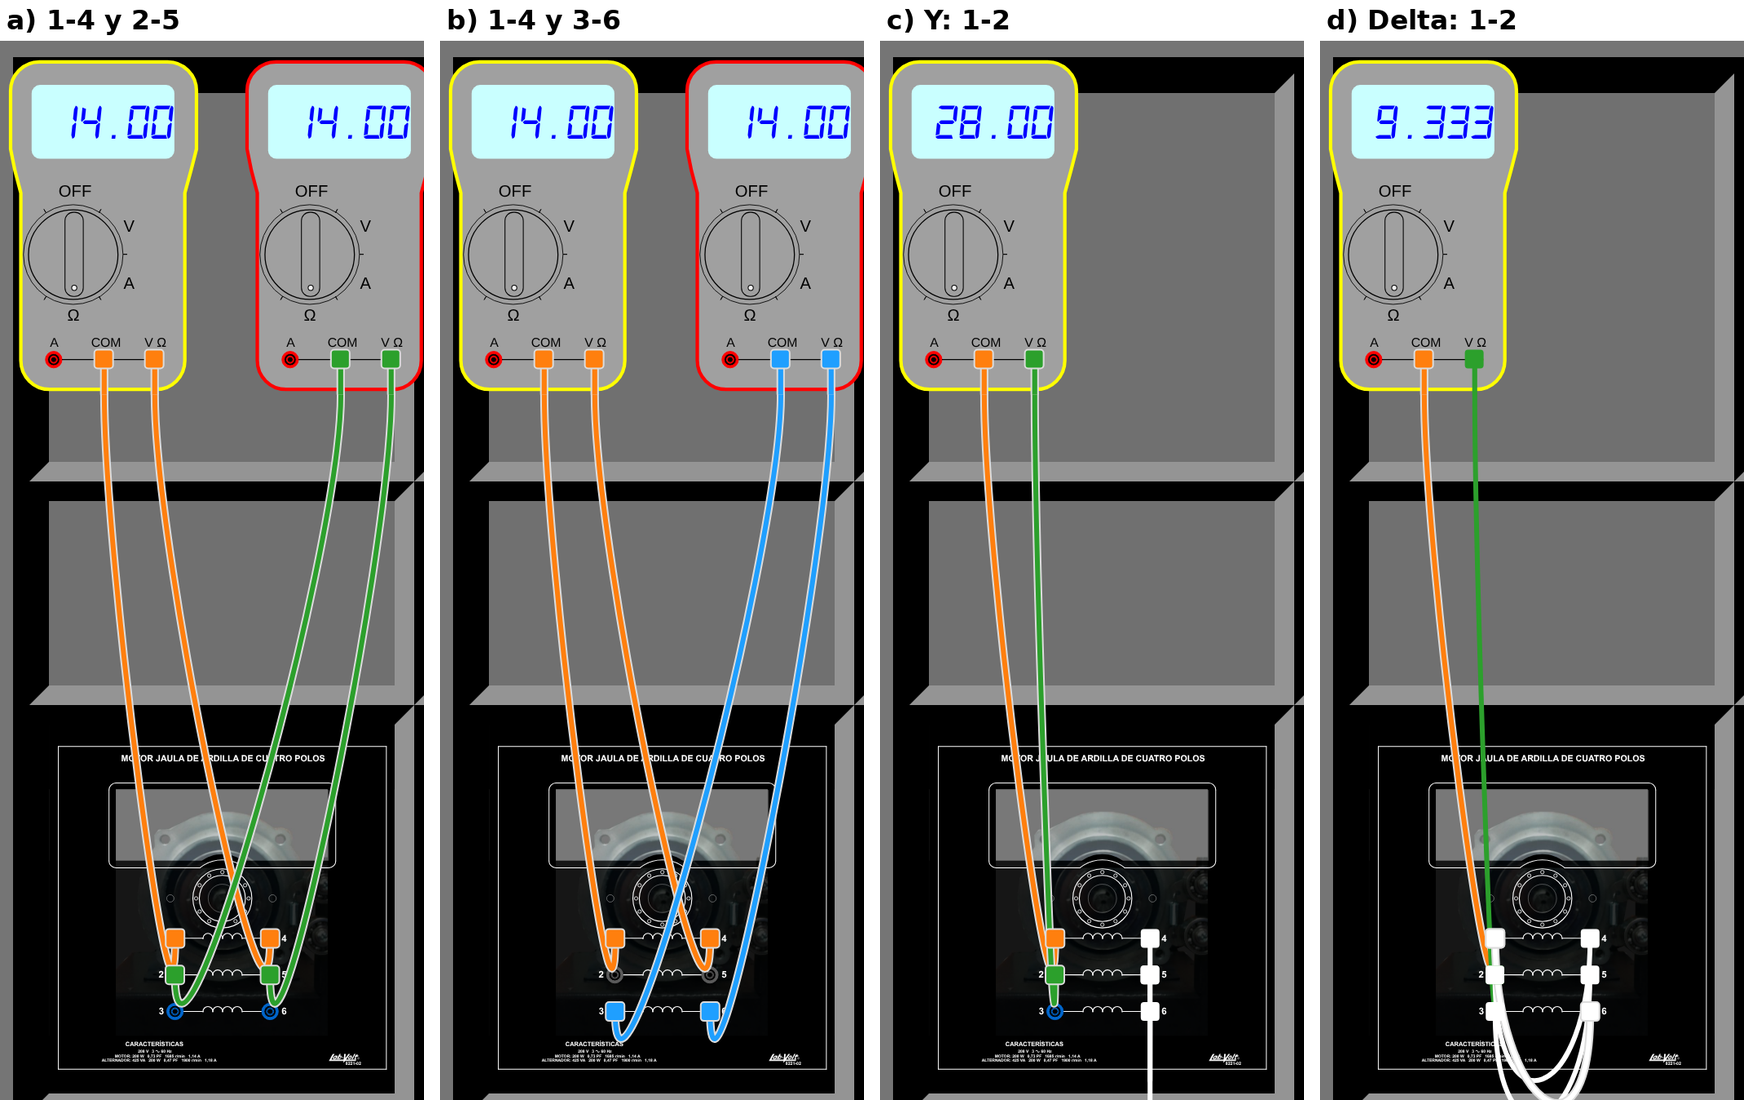
\includegraphics[width=0.8\textwidth]{figuras/lvsim/a11_ohmetro.png}
\caption{Actividad 1.1 en LVSIM. Óhmetros sobre las fases (a) 1--4 y 2--5, (b) 1--4 y 3--6; resistencia entre líneas 1--2 con el estator en (c) estrella y (d) delta.}
\label{fig:a11}
\end{figure*}

\begin{figure}[!t]
\centering
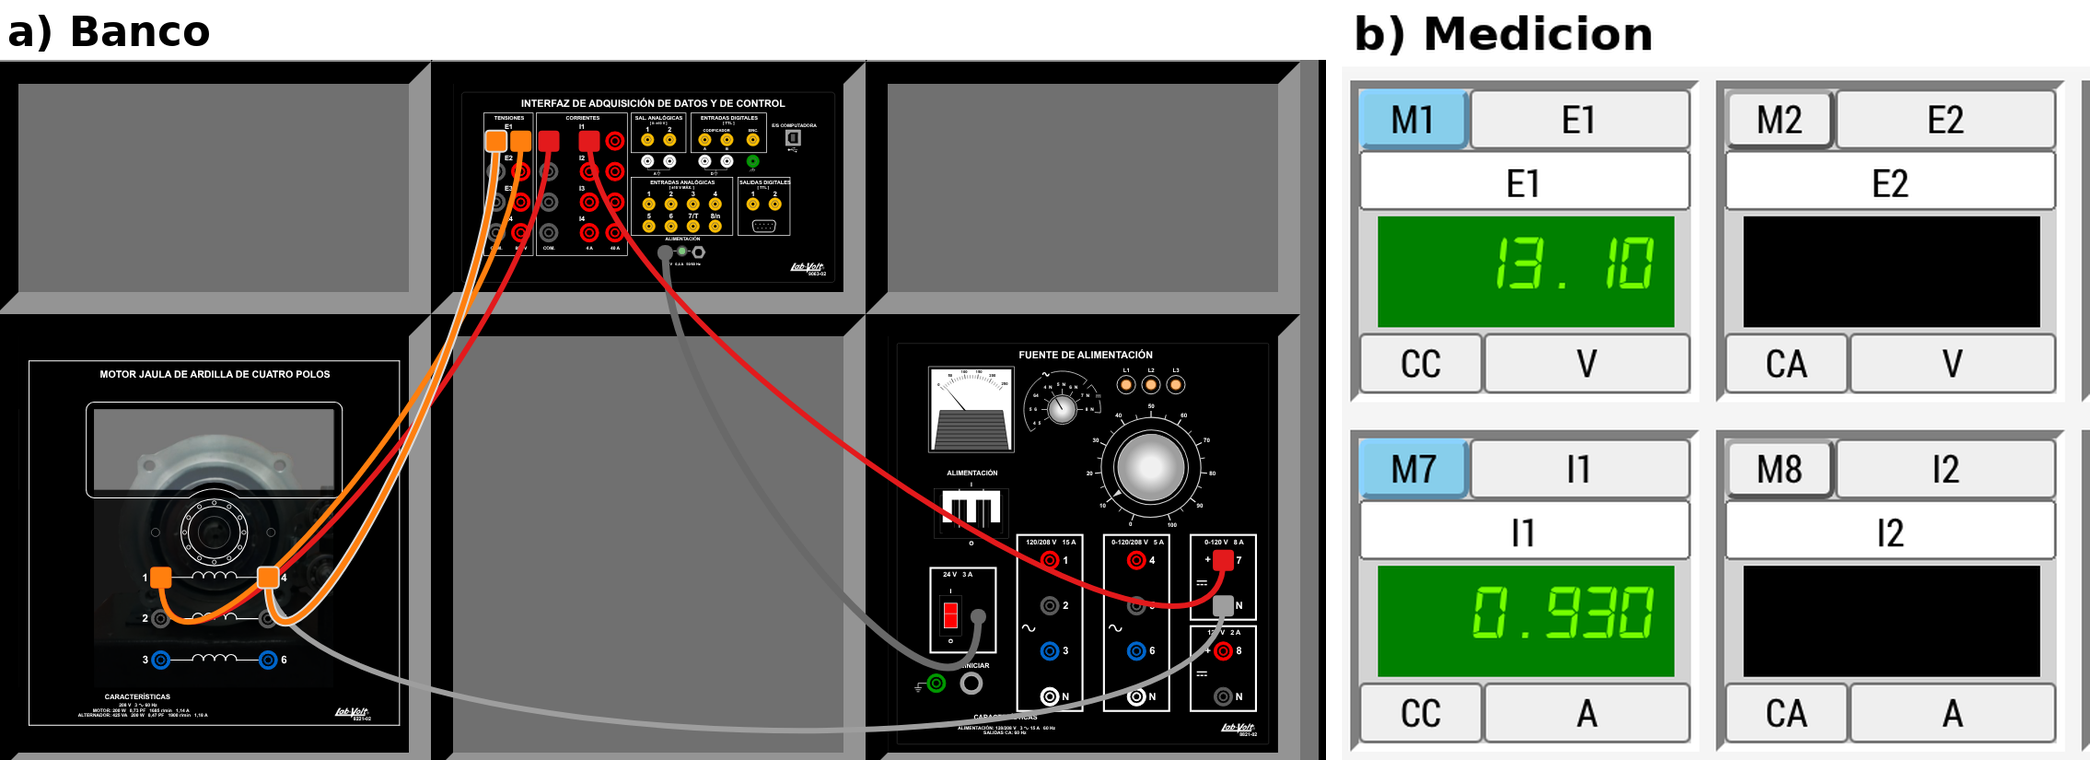
\includegraphics[width=\columnwidth]{figuras/lvsim/a11_voltamperimetrico.png}
\caption{Método voltímetro-amperímetro en CC sobre la fase 1--4 en LVSIM: (a) banco, (b) lectura de E1 e I1 en CC con la perilla de la fuente al \SI{10}{\percent}.}
\label{fig:a11vi}
\end{figure}

\begin{table}[!t]
\centering
\caption{Método voltímetro-amperímetro en CC (fase 1--4, LVSIM)}
\label{tab:vi}
\footnotesize
\begin{tabular}{@{}ccc@{}}
\toprule
$V$ [V] & $I$ [A] & $R=V/I$ [\si{\ohm}] \\
\midrule
\csname @@input\endcsname calculos/salidas/tab_resistencia_cc.tex 
\bottomrule
\end{tabular}
\end{table}

\subsection{Actividad 1.2: puesta en operación}
El motor se conectó en estrella y se alimentó al 100, 80 y 60~\% de \SI{208}{V}; luego se repitió en delta con \SI{120}{V} como tensión nominal (Fig.~\ref{fig:a12}a--b). Para la secuencia se apagó la fuente, se intercambiaron L1 y L2 (secuencia BAC) y, después, L2 y L3 (BCA) (Fig.~\ref{fig:a12}c). La Tabla~\ref{tab:op} resume las corridas. El signo de la velocidad entregado por el dinamómetro indica el sentido de giro: positivo para la secuencia ABC (sentido directo) y negativo para el inverso.

\begin{table*}[!t]
\centering
\caption{Puesta en operación del motor de jaula 8221 en vacío (LVSIM)}
\label{tab:op}
\footnotesize
\begin{tabular}{@{}cccccccccc@{}}
\toprule
Conexión & Secuencia & \% de $V_n$ & $V_L$ [V] & $I_L$ [A] & $P=P_{W1}+P_{W2}$ [W] & $n$ [\si{\rpm}] & $s$ [\%] & Sentido \\
\midrule
\csname @@input\endcsname calculos/salidas/tab_operacion.tex 
\bottomrule
\end{tabular}
\end{table*}

\begin{figure*}[!p]
\centering
\subfloat[Estrella a \SI{208}{V}, secuencia ABC: banco con el dinamómetro como tacómetro y lecturas.\label{fig:a12y}]{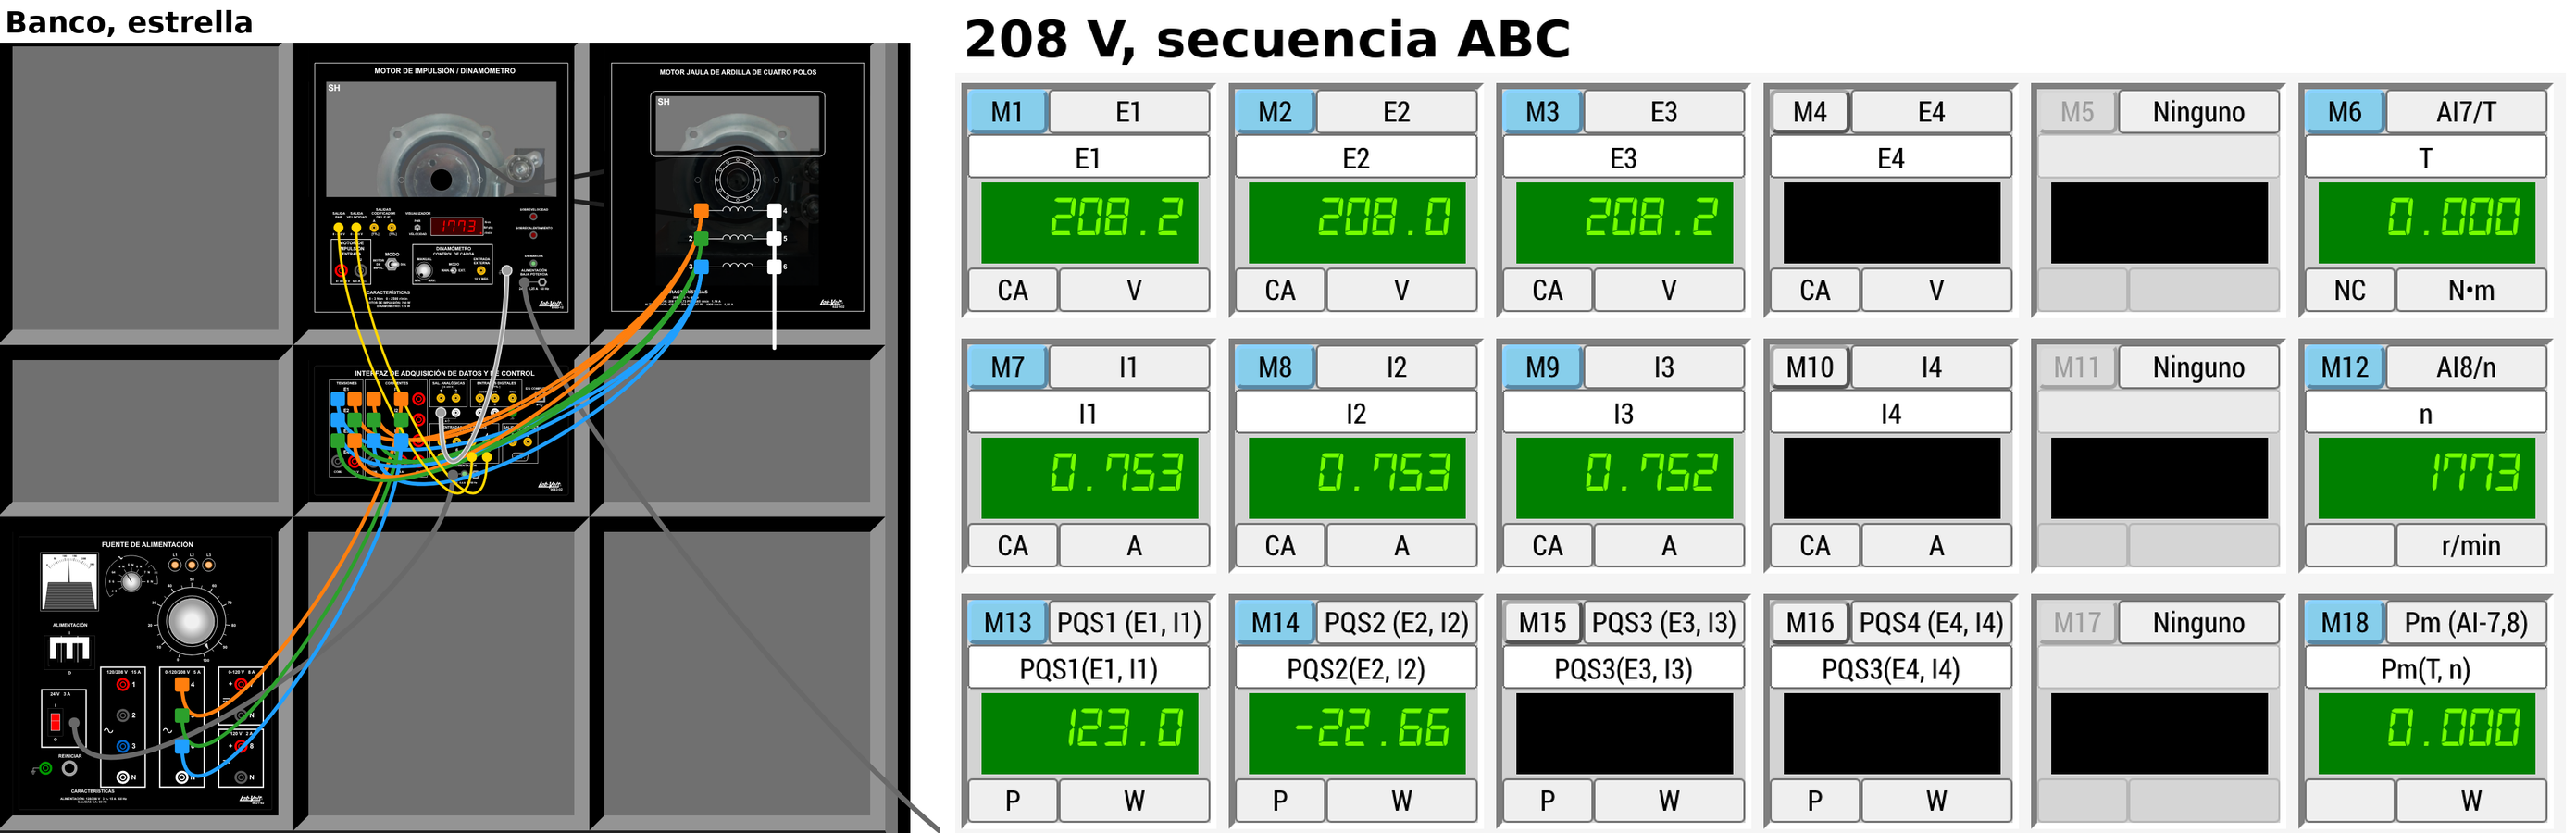
\includegraphics[width=0.86\textwidth]{figuras/lvsim/a12_estrella.png}}\\
\subfloat[Delta a \SI{120}{V}, secuencia ABC: banco y lecturas.\label{fig:a12d}]{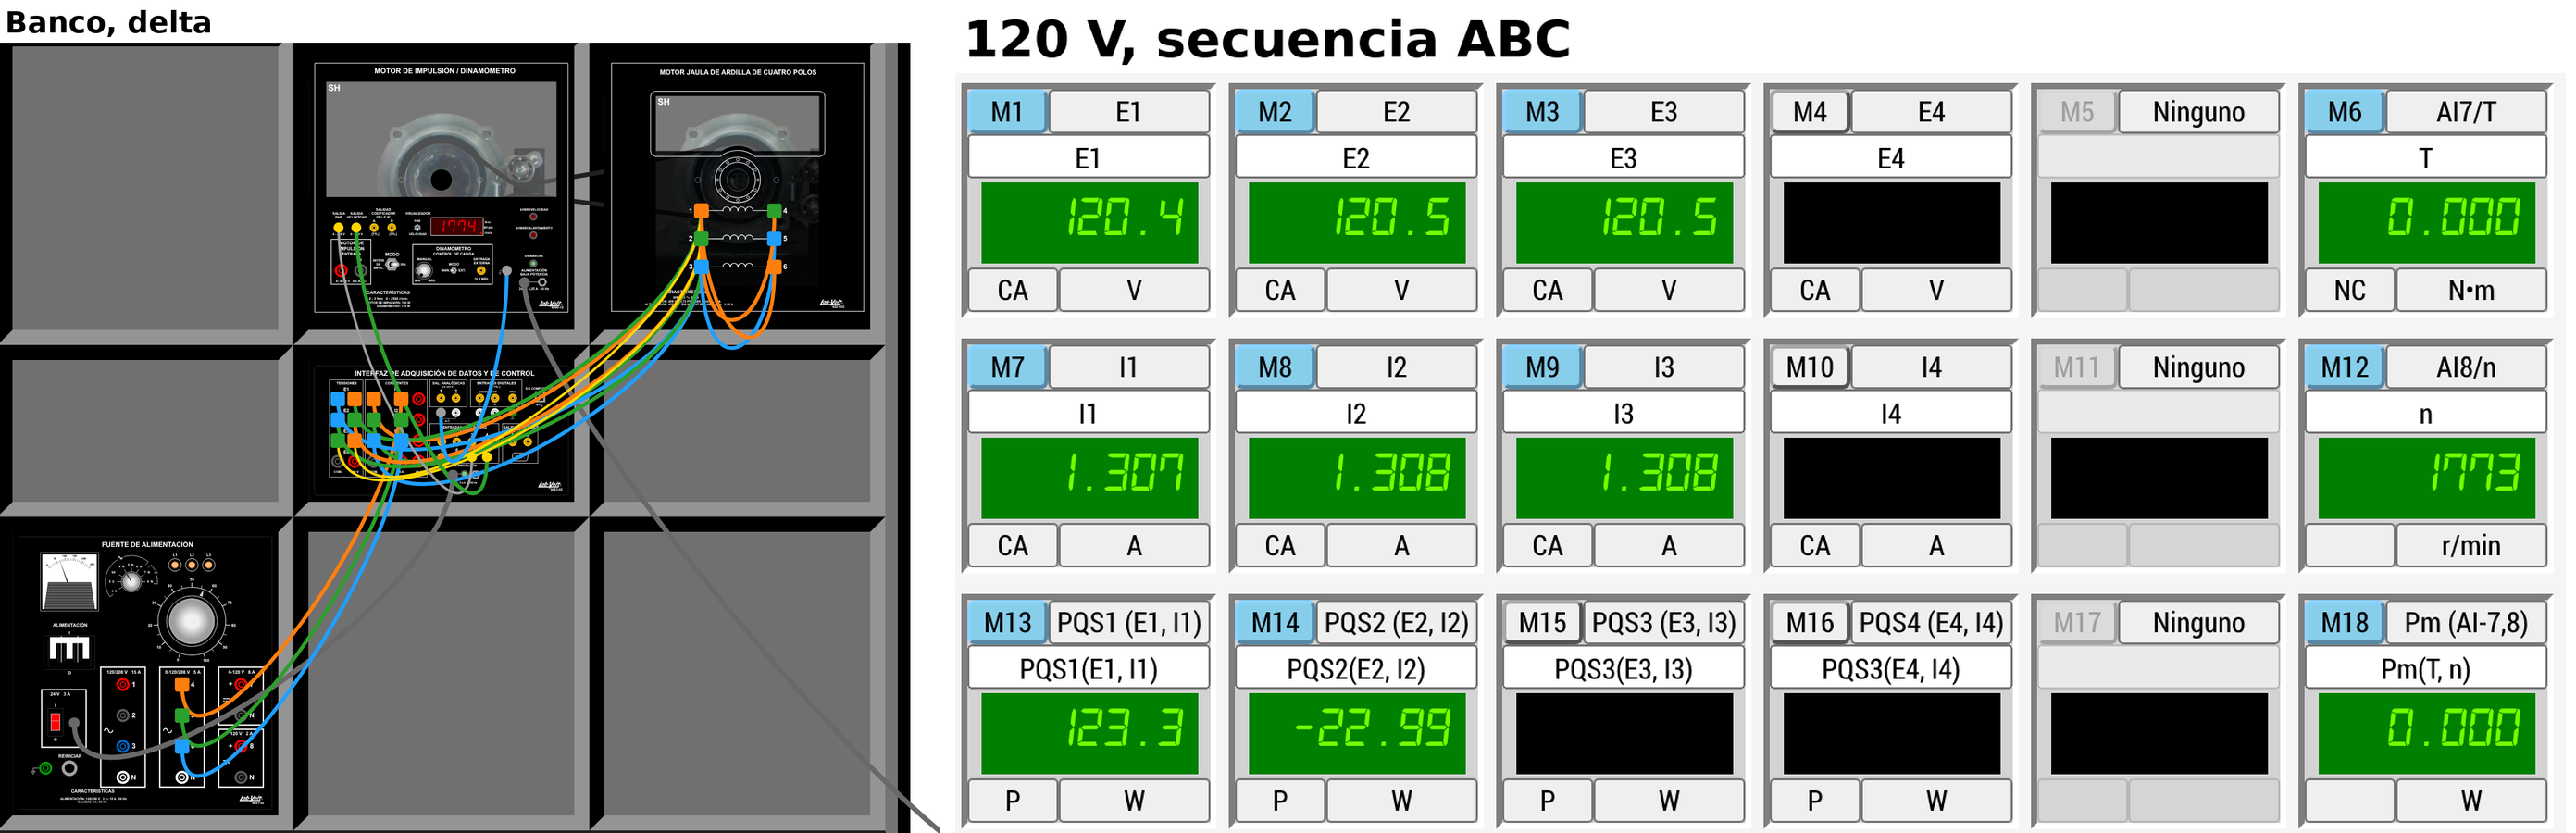
\includegraphics[width=0.86\textwidth]{figuras/lvsim/a12_delta.png}}\\
\subfloat[Estrella a \SI{208}{V} con L1 y L2 intercambiadas ($n=\SI{-1773}{\rpm}$) y luego también L2 y L3 ($n=\SI{1773}{\rpm}$).\label{fig:a12s}]{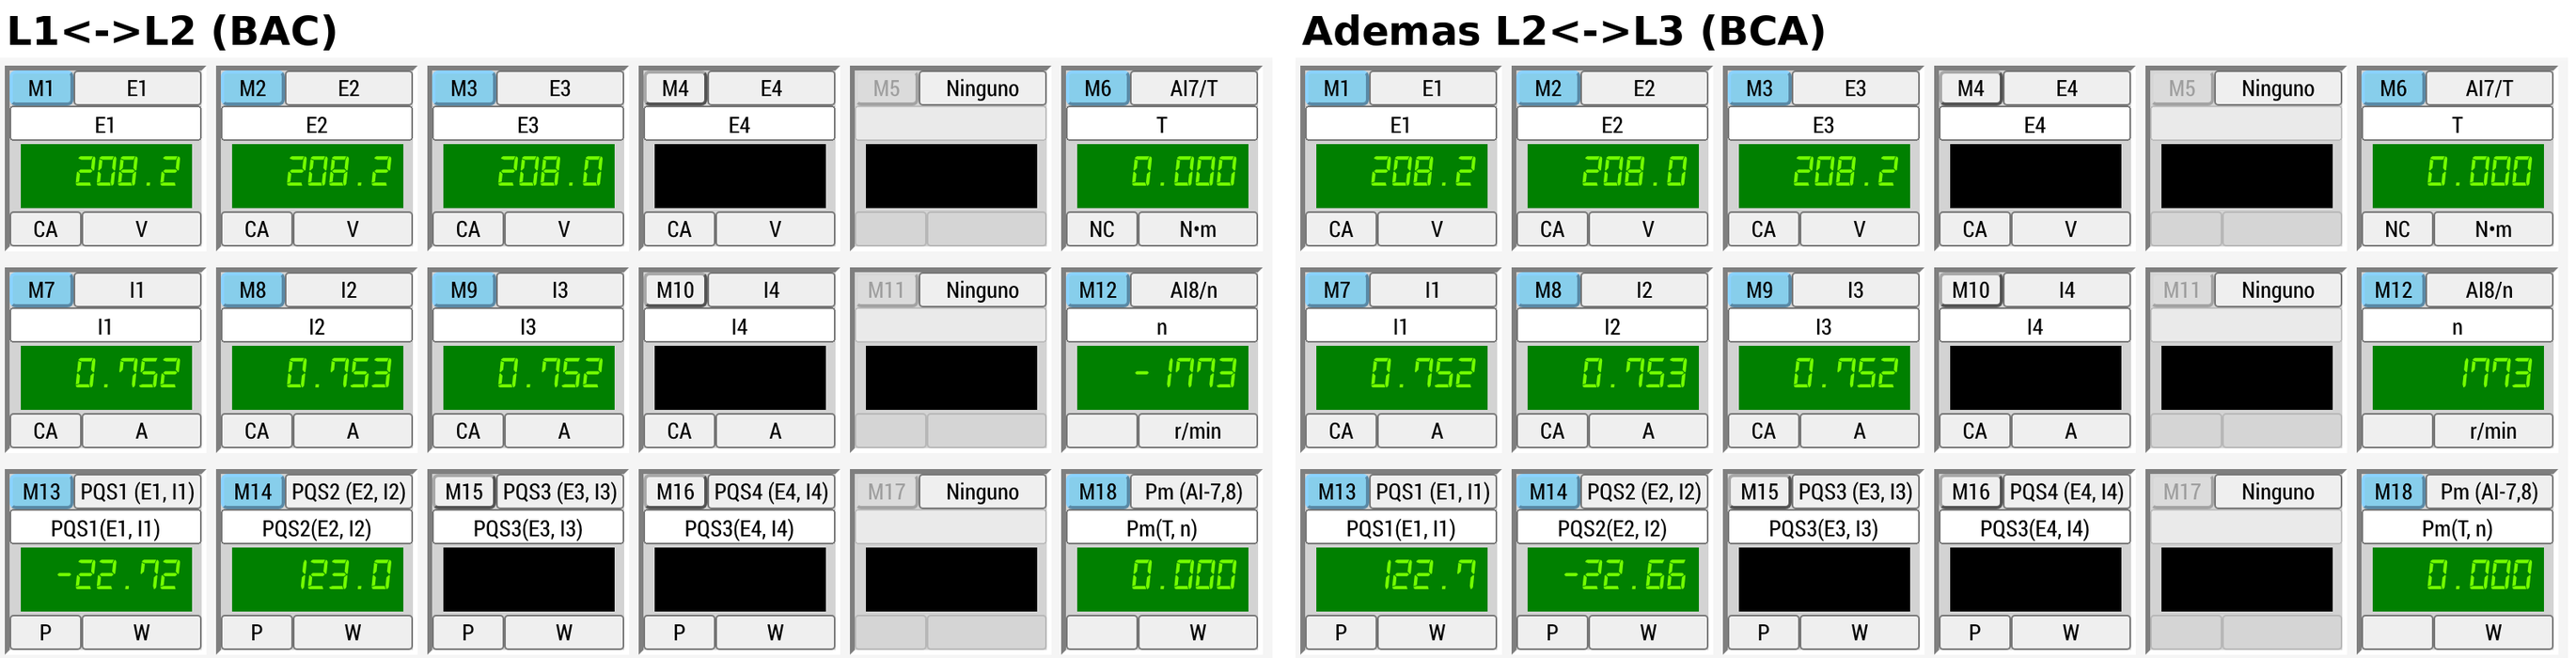
\includegraphics[width=0.86\textwidth]{figuras/lvsim/a12_sentido.png}}
\caption{Actividad 1.2 (puesta en operación) en LVSIM.}
\label{fig:a12}
\end{figure*}

Además se hizo una sola lectura breve con el estator en delta a \SI{208}{V}, para cuantificar el error de usar la tensión de estrella en delta: la corriente de línea llegó a \DdosIL~\si{A} (\DdosIF~\si{A} por bobina, por encima de los \SI{1,5}{A} marcados en el módulo) y la potencia absorbida en vacío a \DdosP~\si{W}, tres veces la de la conexión correcta.

\subsection{Actividad 2.1: prueba de vacío}
Con el motor en delta y sin carga se barrió la tensión según la Tabla~\ref{tab:tensiones} (Fig.~\ref{fig:a2v}). La Tabla~\ref{tab:vacio} es la Tabla~20 de la guía adaptada, con columnas para $P_{Cu}$ y la velocidad. Las Figs.~\ref{fig:vacioP} y~\ref{fig:vacioI} son las gráficas pedidas de potencia y corriente contra tensión, y la Fig.~\ref{fig:vacioV2} separa las pérdidas.

\begin{figure*}[!t]
\centering
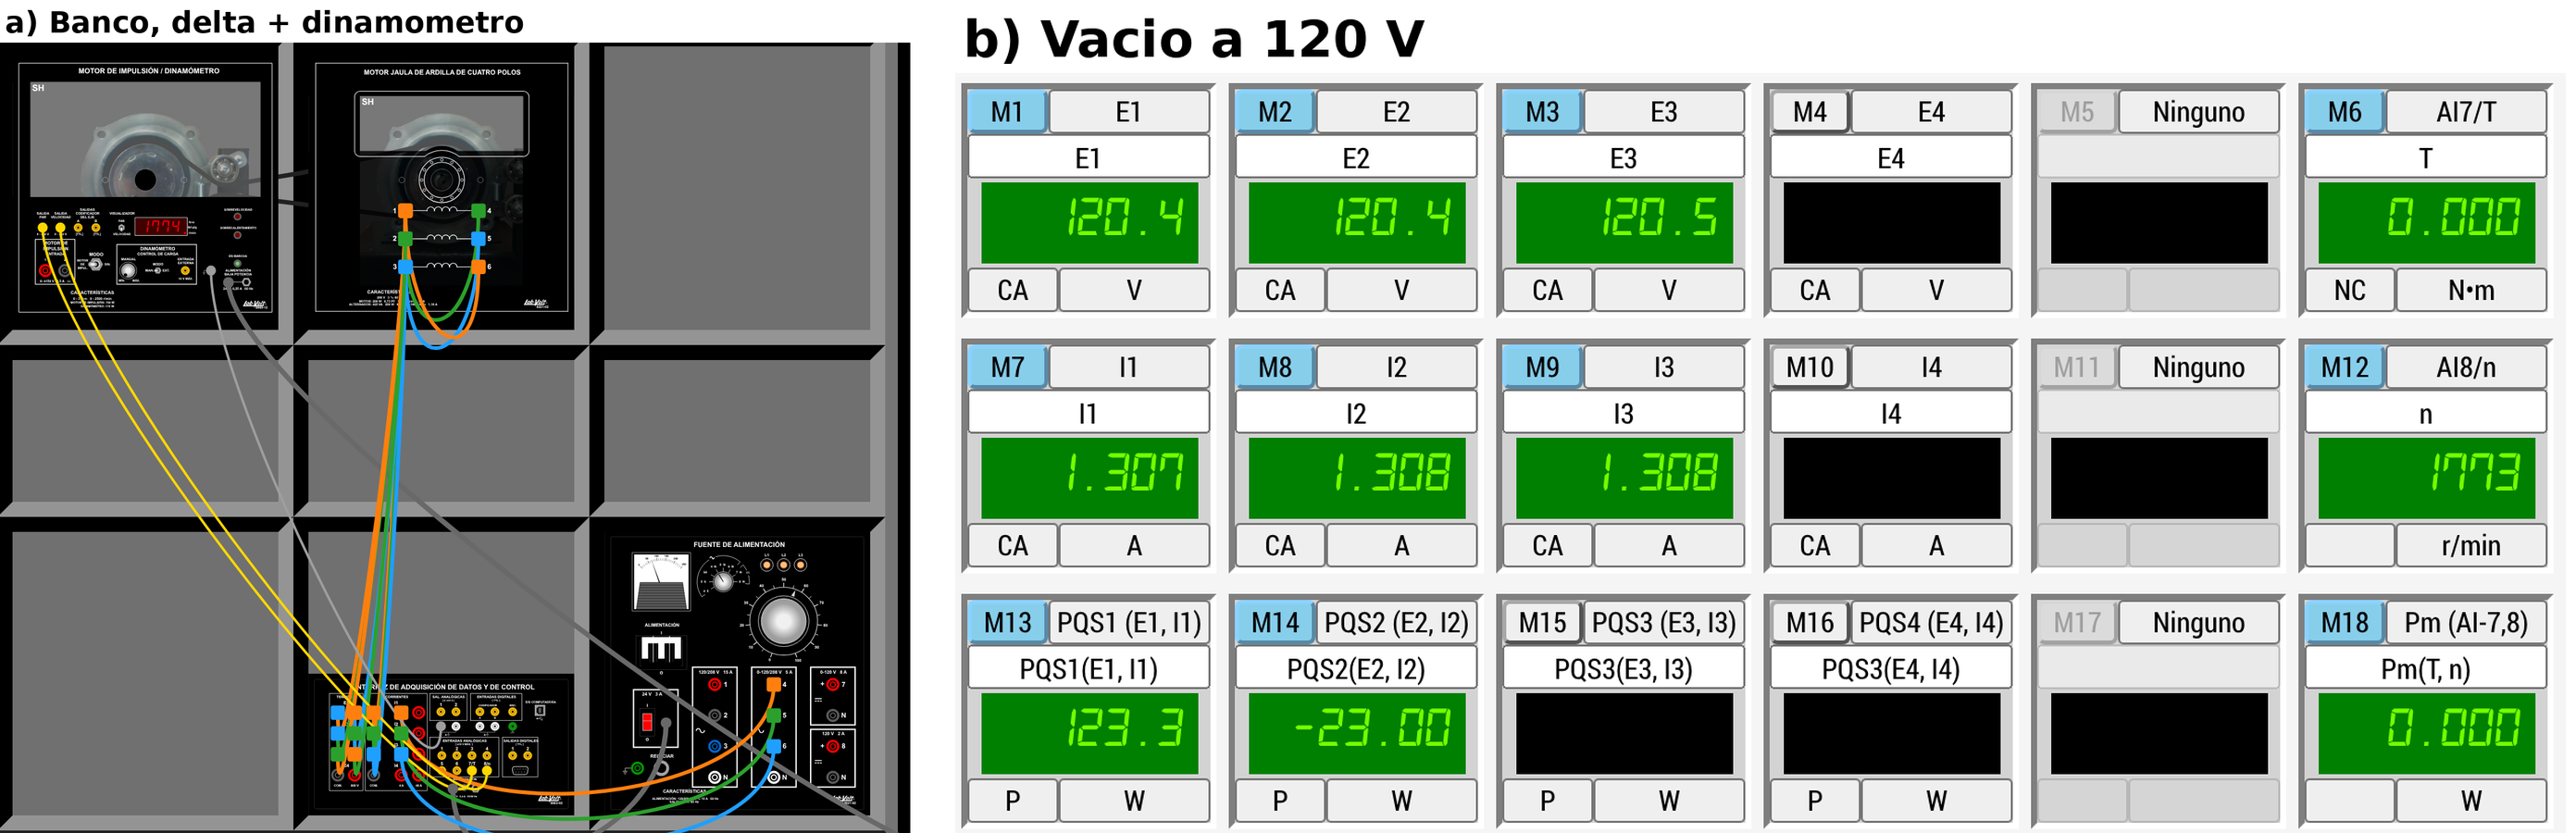
\includegraphics[width=0.9\textwidth]{figuras/lvsim/a2_vacio.png}
\caption{Actividad 2.1 en LVSIM: (a) banco en delta con dos vatímetros (E1/I1, E2/I2) y dinamómetro acoplado sin carga; (b) lecturas a \SI{120}{V}. $P_{W2}$ es negativo porque el factor de potencia en vacío es menor que 0,5.}
\label{fig:a2v}
\end{figure*}

\begin{table*}[!t]
\centering
\caption{Prueba de vacío del motor 8221 en delta (Tabla 20 adaptada, LVSIM). $R_{est}=\SI{14}{\ohm}$, $I_\phi=I_L/\sqrt3$}
\label{tab:vacio}
\footnotesize
\begin{tabular}{@{}ccccccccc@{}}
\toprule
$V_{CA}$ [V] & $I_{CA}$ [A] & $P_{W1}$ [W] & $P_{W2}$ [W] & $P_0$ [W] & $P_{Cu}$ [W] & $P_m+P_{fe}$ [W] & $\cos\theta$ & $n$ [\si{\rpm}] \\
\midrule
\csname @@input\endcsname calculos/salidas/tab_vacio.tex 
\bottomrule
\end{tabular}
\end{table*}

\begin{figure}[!t]
\centering
\begin{tikzpicture}
\begin{axis}[lab,xlabel={$V_{CA}$ [V]},ylabel={Potencia [W]},legend pos=north west,ymin=0]
\addplot+[mark=*,thick] table[x=V,y=P0]{calculos/salidas/vacio.dat};
\addplot+[mark=square*,thick] table[x=V,y=Prot]{calculos/salidas/vacio.dat};
\addplot+[mark=triangle*,thick] table[x=V,y=Pcu]{calculos/salidas/vacio.dat};
\legend{$P_0$,$P_m+P_{fe}$,$P_{Cu}$}
\end{axis}
\end{tikzpicture}
\caption{Prueba de vacío: potencia de entrada y su descomposición contra la tensión de línea (LVSIM).}
\label{fig:vacioP}
\end{figure}

\begin{figure}[!t]
\centering
\begin{tikzpicture}
\begin{axis}[lab,width=0.86\columnwidth,xlabel={$V_{CA}$ [V]},ylabel={$I_{CA}$ [A]},
  axis y line*=left,ymin=0.8,ymax=1.5]
\addplot+[mark=*,thick] table[x=V,y=I]{calculos/salidas/vacio.dat};\label{pl:i}
\end{axis}
\begin{axis}[lab,width=0.86\columnwidth,axis y line*=right,axis x line=none,ylabel={$\cos\theta$},ymin=0.3,ymax=0.9,grid=none,legend pos=north east]
\addplot+[mark=square*,thick,red,dashed,mark options={solid}] table[x=V,y=fp]{calculos/salidas/vacio.dat};
\addlegendimage{/pgfplots/refstyle=pl:i}\addlegendentry{$I_{CA}$}
\addlegendentry{$\cos\theta$}
\end{axis}
\end{tikzpicture}
\caption{Prueba de vacío: corriente de línea y factor de potencia contra la tensión (LVSIM).}
\label{fig:vacioI}
\end{figure}

\begin{figure}[!t]
\centering
\begin{tikzpicture}
\begin{axis}[lab,xlabel={$V_{CA}^2$ [V$^2$]},ylabel={$P_m+P_{fe}$ [W]},legend pos=south east,
  xmin=0,ymin=50,scaled x ticks=base 10:-3,xtick scale label code/.code={$\times10^{3}$}]
\addplot+[only marks,mark=*] table[x=V2,y=Prot]{calculos/salidas/vacio.dat};
\addplot+[no marks,thick,dashed] table[x=V2,y=Prot]{calculos/salidas/vacio_ajuste.dat};
\legend{LVSIM,ajuste ($V\geq\SI{85}{V}$)}
\end{axis}
\end{tikzpicture}
\caption{Pérdidas rotacionales contra $V^2$. La extrapolación a $V=0$ da las pérdidas mecánicas, $P_m\approx\Pmec$~\si{W}.}
\label{fig:vacioV2}
\end{figure}

\subsection{Actividad 2.2: prueba de carga}
Con el motor en delta a \SI{120}{V} se aumentó el par del dinamómetro por pasos y, en cada paso, se reajustó la fuente para devolver la tensión a \SI{120}{V}, como pide la guía. La prueba terminó al pasar la corriente nominal en delta (\LVIfD~\si{A}). La Fig.~\ref{fig:a2c} muestra el punto más cercano a esa corriente y la Tabla~\ref{tab:carga} es la Tabla~21 adaptada. La potencia de salida se calculó con \eqref{eq:eta}; difiere en menos de \CerrPm~\si{W} del medidor Pm(T,n) de LVSIM.

\begin{figure*}[!t]
\centering
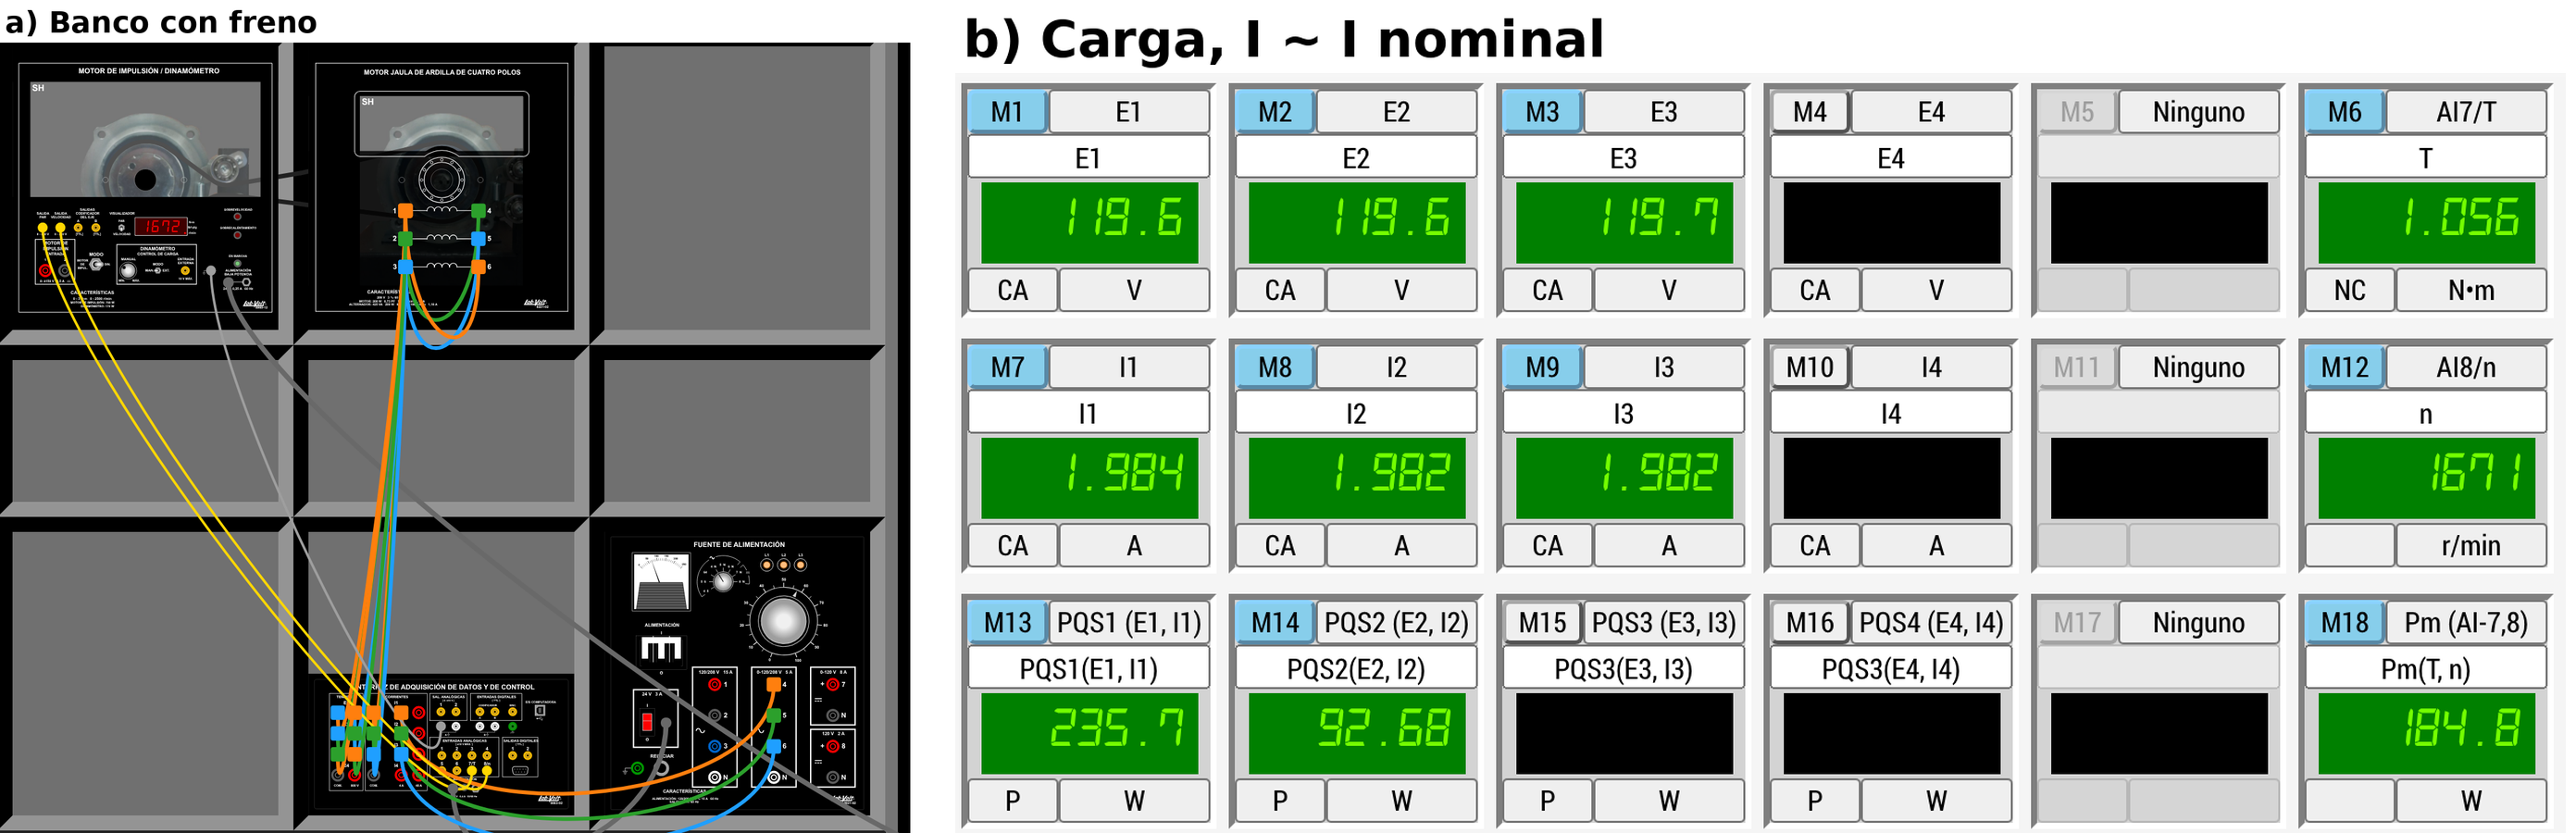
\includegraphics[width=0.9\textwidth]{figuras/lvsim/a2_carga.png}
\caption{Actividad 2.2 en LVSIM: (a) banco con el dinamómetro como freno, (b) lecturas con corriente cercana a la nominal: $\tau=\SI{1,056}{N.m}$, $n=\SI{1671}{\rpm}$, $P_{out}=\SI{184,8}{W}$.}
\label{fig:a2c}
\end{figure*}

\begin{table*}[!t]
\centering
\caption{Prueba de carga del motor 8221 en delta a \SI{120}{V} (Tabla 21 adaptada, LVSIM)}
\label{tab:carga}
\footnotesize
\begin{tabular}{@{}ccccccccc@{}}
\toprule
$I$ [A] & Carga [\%] & $\tau$ [N\,m] & $n$ [\si{\rpm}] & $P_{in}$ [W] & $P_{out}$ [W] & $\eta$ [\%] & $s$ [\%] & $\cos\theta$ \\
\midrule
\csname @@input\endcsname calculos/salidas/tab_carga.tex 
\bottomrule
\end{tabular}
\end{table*}

\begin{figure}[!t]
\centering
\subfloat[Velocidad contra par]{%
\begin{tikzpicture}
\begin{axis}[lab,width=0.52\columnwidth,height=0.48\columnwidth,xlabel={$\tau$ [N\,m]},ylabel={$n$ [\si{\rpm}]}]
\addplot+[mark=*,thick] table[x=tau,y=n]{calculos/salidas/carga.dat};
\end{axis}
\end{tikzpicture}}\hfill
\subfloat[Velocidad contra corriente]{%
\begin{tikzpicture}
\begin{axis}[lab,width=0.52\columnwidth,height=0.48\columnwidth,xlabel={$I$ [A]},ylabel={$n$ [\si{\rpm}]}]
\addplot+[mark=*,thick] table[x=I,y=n]{calculos/salidas/carga.dat};
\end{axis}
\end{tikzpicture}}\\
\subfloat[Eficiencia contra par]{%
\begin{tikzpicture}
\begin{axis}[lab,width=0.52\columnwidth,height=0.48\columnwidth,xlabel={$\tau$ [N\,m]},ylabel={$\eta$ [\%]},ymin=0]
\addplot+[mark=*,thick] table[x=tau,y=eta]{calculos/salidas/carga.dat};
\end{axis}
\end{tikzpicture}}\hfill
\subfloat[Eficiencia contra $P_{out}$]{%
\begin{tikzpicture}
\begin{axis}[lab,width=0.52\columnwidth,height=0.48\columnwidth,xlabel={$P_{out}$ [W]},ylabel={$\eta$ [\%]},ymin=0]
\addplot+[mark=*,thick] table[x=Pout,y=eta]{calculos/salidas/carga.dat};
\end{axis}
\end{tikzpicture}}\\
\subfloat[Deslizamiento contra $P_{out}$]{%
\begin{tikzpicture}
\begin{axis}[lab,width=0.52\columnwidth,height=0.48\columnwidth,xlabel={$P_{out}$ [W]},ylabel={$s$ [\%]},ymin=0]
\addplot+[mark=*,thick] table[x=Pout,y=s]{calculos/salidas/carga.dat};
\end{axis}
\end{tikzpicture}}\hfill
\subfloat[Factor de potencia contra $P_{out}$]{%
\begin{tikzpicture}
\begin{axis}[lab,width=0.52\columnwidth,height=0.48\columnwidth,xlabel={$P_{out}$ [W]},ylabel={$\cos\theta$}]
\addplot+[mark=*,thick] table[x=Pout,y=fp]{calculos/salidas/carga.dat};
\end{axis}
\end{tikzpicture}}
\caption{Curvas de la prueba de carga (LVSIM, delta, \SI{120}{V}).}
\label{fig:curvascarga}
\end{figure}

\FloatBarrier
% ===========================================================================
\section{Procedimiento y seguridad}
\begin{enumerate}
\item Antes de energizar, leer la placa real de cada motor y anotar tensión, corriente, potencia y velocidad para cada conexión. Confirmar que la tensión de línea elegida corresponde a la conexión (en el DL~1021, \SI{220}{V} en delta o \SI{380}{V} en estrella).
\item Fijar el motor a la base y comprobar que el eje gire libre y que el acople con el freno esté protegido.
\item Medir resistencias con el motor desenergizado y sin puentes, y repetir la medida si dos fases difieren más del 3--5~\%.
\item Arrancar siempre desde tensión cero y subirla gradualmente vigilando la corriente. No superar la corriente nominal de la conexión (en el DL~1021, \SI{4,3}{A} en delta). La Tabla~20 pide \SI{240}{V} en delta, el 109~\% de la nominal; ese punto se toma rápido y solo si la corriente lo permite.
\item Toda modificación del montaje (puentes, intercambio de líneas, rotor abierto o en corto) se hace con la fuente apagada.
\item Con el rotor devanado abierto el motor no arranca y el estator absorbe la corriente de magnetización; no dejarlo energizado más de lo necesario para medir la tensión en los anillos.
\item En la prueba de carga, nivelar el freno sin excitación, desplazar la pesa de \SI{2}{cm} en \SI{2}{cm}, mantener la tensión nominal y detenerse al llegar a la corriente nominal.
\item No tocar el eje, el acople ni la correa con el motor en giro. Usar el tacómetro óptico a distancia.
\end{enumerate}

% ===========================================================================
\section{Análisis de resultados}
\label{sec:analisis}

\subsection{Resistencia de los devanados}
Las tres fases del 8221 tienen la misma resistencia, como corresponde a un estator simétrico. El método voltímetro-amperímetro da \Rvi~\si{\ohm}, un 1~\% por encima del óhmetro; el intercepto casi nulo indica que no hay caída de tensión fija en el circuito y que la diferencia se debe a la resolución de los medidores a corrientes bajas. Las medidas entre líneas ($2R$ en estrella, $2R/3$ en delta) comprueban que los puentes estaban bien hechos, una verificación útil antes de energizar en el banco físico. Allí la resistencia será menor: un motor de \SI{1,1}{kW} tiene conductores más gruesos que uno de \SI{200}{W}. Además se medirá a temperatura ambiente; para estimar las pérdidas a temperatura de operación habría que corregir la resistencia por temperatura \cite{ieee112}.

Entre los motores, el de rotor devanado tiene una resistencia rotórica medible y mayor que la de la jaula, porque su rotor tiene bobinas de muchas espiras de alambre fino conectadas a través de escobillas y anillos, mientras que la jaula está formada por barras gruesas en cortocircuito. Esa mayor resistencia de rotor le da más par de arranque y más deslizamiento a plena carga.

\subsection{Puesta en operación}
\textbf{Rotor devanado (análisis teórico).} Con los anillos abiertos el motor no gira: no circula corriente en el rotor y no hay par. El estator crea igualmente el campo giratorio, que induce en el rotor detenido la tensión $E_{R0}$ a la frecuencia de la red, como en un transformador en vacío; por eso sí hay tensión entre los anillos. Al unir los anillos circula corriente rotórica y el motor arranca. Si en lugar de un corto se conectara una resistencia trifásica, el arranque sería más suave y con más par.

\textbf{Sentido de giro.} En LVSIM, con la secuencia ABC la velocidad es positiva; al intercambiar L1 y L2 se vuelve negativa ($-1773$~\si{\rpm}), y al intercambiar después L2 y L3 vuelve a ser positiva. La razón es que cada intercambio de dos líneas invierte la secuencia de fases y con ella el sentido del campo giratorio; dos intercambios sucesivos restauran la secuencia original (BCA es una rotación de ABC). Las magnitudes eléctricas no cambian, solo se intercambian las lecturas de los dos vatímetros. En el banco físico esto se verificará en ambos motores y en ambas conexiones.

\textbf{Tensión reducida.} En los dos casos la velocidad baja de \SI{1773}{\rpm} al 100~\% a unos \SI{1720}{\rpm} al 60~\%; el deslizamiento pasa de 1,5~\% a cerca de 4,5~\%. Como el par disponible es proporcional a $V^2$, el motor necesita más deslizamiento para producir el mismo par de fricción. La tendencia es la que predice la Sección~VII-F, aunque los valores son menores porque el par en vacío es solo el de fricción. La corriente baja al reducir la tensión porque baja la corriente de magnetización.

\textbf{Estrella frente a delta.} El motor en estrella a \SI{208}{V} y en delta a \SI{120}{V} tiene la misma potencia, velocidad y deslizamiento, y la corriente de línea en delta es $\sqrt3$ veces la de estrella ($1{,}308/0{,}753=1{,}74$). En ambos casos cada bobina recibe \SI{120}{V}, así que el motor opera igual. La lectura en delta a \SI{208}{V} muestra lo contrario: \DdosIF~\si{A} por bobina y el triple de potencia en vacío, por saturación del núcleo. En el banco físico, el DL~1021 debe ir en delta a \SI{220}{V} y en estrella a \SI{380}{V}.

\subsection{Prueba de vacío}
A tensión nominal el motor absorbe \InomVac~\si{A} con $\cos\theta=\FPnomVac$. La corriente en vacío es el 66~\% de la nominal (\LVIfD~\si{A}): es casi toda corriente de magnetización, necesaria porque el circuito magnético tiene entrehierro. Por eso el factor de potencia en vacío es bajo y el segundo vatímetro marca negativo para $V\geq\SI{98}{V}$, lo que corresponde a $\cos\theta<0{,}5$.

De los \PceroNom~\si{W} absorbidos a \VnomVac~\si{V}, \PcuNom~\si{W} son pérdidas en el cobre del estator y \ProtNom~\si{W} pérdidas rotacionales. La recta de la Fig.~\ref{fig:vacioV2} separa estas últimas en \Pmec~\si{W} mecánicas y \PfeNom~\si{W} en el hierro, con lo cual se cumple la igualdad de la guía:
\[
P_0=P_{Cu}+P_m+P_{fe}=\PcuNom+\Pmec+\PfeNom\approx\PceroNom~\si{W}.
\]
Las pérdidas mecánicas resultan altas porque el dinamómetro quedó acoplado por correa y su fricción se suma a la del motor; en el banco físico se debe desacoplar el freno para la prueba de vacío. Para tensiones por debajo de unos \SI{75}{V} la corriente vuelve a subir: el par de fricción obliga a aumentar el deslizamiento ($n$ cae a \SI{1649}{\rpm} a \SI{55}{V}) y crece la componente activa de la corriente del rotor. Esos puntos se excluyeron del ajuste lineal.

Con los valores a tensión nominal, la rama de magnetización vista por fase vale aproximadamente $Z_0=V_\phi/I_\phi=\Zvac$~\si{\ohm}, que es casi toda $X_1+X_M$ porque $R_1=\SI{14}{\ohm}$, y $R_c\approx V_\phi^2/(P_{fe}/3)\approx\Rfe$~\si{\ohm}. Para completar el circuito equivalente faltaría la prueba de rotor bloqueado, que la guía no incluye.

\subsection{Prueba de carga}
Al aumentar la carga, la velocidad baja casi linealmente de \Cnvac~\si{\rpm} a \Cnomn~\si{\rpm} con corriente nominal (Fig.~\ref{fig:curvascarga}a). Esta es la zona estable de la curva par-velocidad, cerca de $n_s$, donde el par es proporcional al deslizamiento. La regulación de velocidad, con \eqref{eq:rv}, es \CRV~\%. La corriente sube desde el valor de vacío porque se suma la componente activa que exige el par (Fig.~\ref{fig:curvascarga}b).

Con corriente nominal (\CnomI~\si{A}) el motor entrega \CnomPout~\si{W}, con $\tau=\CnomT$~\si{N.m}, $s=\Cnoms$~\% y $\eta=\Cnometa$~\%. La eficiencia crece rápido con la carga, porque las pérdidas fijas pesan menos, y se aplana hacia el \SI{57}{\percent} (Fig.~\ref{fig:curvascarga}c--d). El factor de potencia pasa de 0,37 en vacío a \Cnomfp\ con corriente nominal (Fig.~\ref{fig:curvascarga}f): al crecer la componente activa de la corriente, la reactiva de magnetización pesa menos. El deslizamiento crece de forma casi proporcional a la potencia entregada (Fig.~\ref{fig:curvascarga}e), como lo indica $P_{Cu2}=sP_{AG}$.

El balance de potencias con corriente nominal, usando \eqref{eq:flujo1}--\eqref{eq:flujo2}, es: $P_{Cu1}=\CnomPcuu$~\si{W}, $P_{fe}=\PfeNom$~\si{W}, $P_{AG}=\CnomPag$~\si{W}, $P_{Cu2}=sP_{AG}=\CnomPcud$~\si{W} y $P_m=\Pmec$~\si{W}. La suma con $P_{out}$ difiere de $P_{in}$ en \CnomResto~\si{W}, un 2~\% de la entrada. La diferencia se atribuye a que las pérdidas mecánicas se tomaron de la prueba de vacío y a que las del hierro bajan un poco con carga por la caída de tensión en el estator.

\subsection{Comparación con la placa}
La placa del 8221 indica \SI{200}{W} a \SI{1685}{\rpm} y \SI{1,14}{A} (en estrella, equivalente a \LVIfD~\si{A} en delta). En LVSIM, con esa corriente el motor entrega \CnomPout~\si{W} a \Cnomn~\si{\rpm}, y los \SI{200}{W} se alcanzan a unos \SI{2,08}{A} y \SI{1660}{\rpm}. La eficiencia simulada (\Cnometa~\%) es menor que la de placa (\LVeta~\%). Una parte de la diferencia es la fricción del dinamómetro acoplado y otra, el modelo del simulador; en todo caso, la placa da valores nominales de diseño y el ensayo da los del equipo concreto. En el último punto la salida (\CultPout~\si{W}) superó los \SI{175}{W} del dinamómetro como freno; en el banco físico se deben respetar los límites del freno además de los del motor.

\subsection{Por qué el motor de jaula es el más usado}
Las curvas muestran tres características. Primera, velocidad casi constante: entre vacío y plena carga la velocidad cambia menos del \SI{6}{\percent}. Segunda, eficiencia y factor de potencia que mejoran con la carga hasta valores aceptables cerca del punto nominal. Tercera, comportamiento estable: el motor se ajusta solo a la carga, aumentando el deslizamiento sin control externo. A eso se suma la ausencia de escobillas y anillos. El motor de rotor devanado se comporta igual cuando sus anillos están en corto; su ventaja es poder modificar la resistencia rotórica, a cambio de más costo y mantenimiento.

\subsection{Frecuencia del rotor}
Con \eqref{eq:fr} y los datos de LVSIM, la frecuencia del rotor es de \SI{0,9}{Hz} en vacío ($s=1{,}5$~\%) y de unos \SI{4,2}{Hz} con corriente nominal ($s=\Cnoms$~\%), frente a \SI{60}{Hz} con rotor bloqueado. En el motor de rotor devanado esta frecuencia se podría observar en los anillos: es igual a la de la red con el rotor detenido y disminuye a medida que el motor acelera.

\subsection{Observaciones sobre la guía}
\begin{itemize}
\item El cuestionario se titula ``Transformadores Eléctricos''; parece copiado de la práctica anterior. El contenido corresponde a motores de inducción.
\item La guía no indica la referencia del motor de rotor devanado; se supuso el DL~1022.
\item En la lista de pérdidas de la prueba de vacío, ``pérdidas en el marco del estator'' se interpreta como pérdidas en el núcleo (hierro) del estator.
\item La Tabla~20 empieza en \SI{240}{V}, por encima de la tensión nominal en delta del DL~1021 (\SI{220}{V}).
\item La Tabla~21 pide $X$ [m], pero la guía no da la masa de la pesa ni el brazo del freno; se deben leer en el banco para calcular $\tau=mgX$.
\item Los datos de catálogo del DL~1021 son para \SI{50}{Hz}; en Colombia se opera a \SI{60}{Hz} y la velocidad será un 20~\% mayor.
\end{itemize}

% ===========================================================================
\section{Conclusiones}
\begin{itemize}
\item La resistencia por fase del motor simulado es de \SI{14}{\ohm} en las tres fases, y las medidas entre líneas ($2R$ en estrella, $2R/3$ en delta) confirman la teoría y sirven para verificar los puentes antes de energizar.
\item El sentido de giro depende solo de la secuencia de fases: un intercambio de dos líneas lo invierte y un segundo intercambio lo restaura, sin cambiar las magnitudes eléctricas.
\item La conexión correcta depende de la tensión de cada bobina: el motor en delta a \SI{120}{V} opera igual que en estrella a \SI{208}{V}. Alimentar en delta con la tensión de estrella eleva la corriente por bobina por encima de su valor nominal y triplica las pérdidas en vacío.
\item Al reducir la tensión el deslizamiento aumenta, porque el par disponible varía con $V^2$, tal como predice la teoría.
\item En vacío la corriente es principalmente de magnetización y el factor de potencia es bajo (0,37). La potencia absorbida (\PceroNom~\si{W}) se reparte en \PcuNom~\si{W} de cobre, \Pmec~\si{W} mecánicas y \PfeNom~\si{W} de hierro, y la suma coincide con $P_0$, como plantea la guía.
\item Con carga nominal el motor simulado entrega \CnomPout~\si{W} con deslizamiento de \Cnoms~\%, eficiencia de \Cnometa~\% y regulación de velocidad de \CRV~\%. La eficiencia es menor que la de placa porque la fricción del dinamómetro acoplado se suma a las pérdidas.
\item Estos resultados servirán de referencia para el informe final: allí se compararán con los del DL~1021 y el motor de rotor devanado, que trabajan a otra escala de potencia y con 2 polos.
\end{itemize}

% ===========================================================================
\section{Uso de inteligencia artificial}
\nota{Pendiente: redactar según lo que indique Simón.}

% ===========================================================================
\begin{thebibliography}{99}
\bibitem{guia} Universidad del Norte, ``Práctica N.º 4: Máquinas de inducción,'' guía del Laboratorio de Máquinas Eléctricas I, Barranquilla, Colombia.
\bibitem{diapositivas} Universidad del Norte, ``Motor de inducción trifásico,'' diapositivas del curso Máquinas Eléctricas I, periodo 202430.
\bibitem{generador} Universidad del Norte, ``Generador de inducción trifásico: principio de operación, funcionamiento aislado y aplicación en la generación eólica,'' material de apoyo de Máquinas Eléctricas I.
\bibitem{chapman} S.~J. Chapman, \emph{Máquinas eléctricas}, 5.ª ed. México: McGraw-Hill, 2012, cap.~6.
\bibitem{fitzgerald} A.~E. Fitzgerald, C.~Kingsley Jr. y S.~D. Umans, \emph{Electric Machinery}, 6.ª ed. Nueva York: McGraw-Hill, 2003.
\bibitem{ieee112} \emph{IEEE Standard Test Procedure for Polyphase Induction Motors and Generators}, IEEE Std 112-2017, 2018.
\bibitem{lvsim} Festo Didactic, ``LVSIM-EMS: Electromechanical Systems Simulation Software.'' [En línea]. Disponible: \url{https://lvsim.labvolt.com}
\bibitem{lv8221} Festo Didactic (Lab-Volt), ``Four-Pole Squirrel-Cage Induction Motor, model 8221,'' hoja técnica 579491 (120 V, 60 Hz). [En línea]. Disponible: \url{https://www.labvolt.com/downloads/datasheet_579491(50-8221-0)_en_120V_60Hz.pdf}
\bibitem{dl1021} De Lorenzo, ``DL 1021: Motor asíncrono trifásico de jaula de ardilla,'' catálogo de producto. [En línea]. Disponible: \url{https://delorenzoglobal.com/prodotto/motore-asincrono-trifase-a-gabbia-di-scoiattolo-3/}
\bibitem{dl1022} De Lorenzo, ``DL 1022: Motor asíncrono trifásico de anillos,'' catálogo de producto. [En línea]. Disponible: \url{https://delorenzoglobal.com/prodotto/motore-asincrono-trifase-ad-anelli-4/}
\bibitem{img_ksb} KSB Aktiengesellschaft, ``KSB 09 Etanorm mit Motor und Frequenzumrichter,'' Wikimedia Commons, 2009, licencia CC BY-SA 3.0. [En línea]. Disponible: \url{https://commons.wikimedia.org/wiki/File:KSB_09_Etanorm_mit_Motor_und_Frequenzumrichter.jpg}
\bibitem{img_estator} Zureks, ``Stator and rotor by Zureks,'' Wikimedia Commons, 2008, licencia CC BY-SA 3.0. [En línea]. Disponible: \url{https://commons.wikimedia.org/wiki/File:Stator_and_rotor_by_Zureks.JPG}
\end{thebibliography}

\end{document}
